

\input{../Latex_Templates/Preamble_Report}

%%%%% TITLE PAGE

%\subject{, VT23}
\title{ Report for the Course Modelling in Computational Science, HT23 \\[1ex]
	  \large Project 2: Cell reprogramming}
%\subtitle{}
\author{Theo Koppenhöfer \\[1ex] (with Jimmy Gunnarson)}
\date{Lund \\[1ex] \today}

\addbibresource{bibliography.bib}

\usepackage{pythonhighlight}
\usepackage{pgfplots}
\graphicspath{{../Plots/}}

\pgfplotsset{
	compat=newest,
    every axis/.append style={
        axis y line=left,
        axis x line=bottom,
        scale only axis,
%    	max space between ticks=25pt,
        width=0.7\textwidth,
        scaled ticks=true,
        axis line style={thick,-,>=latex, shorten >=-.4cm},
    		x tick label style={
		    /pgf/number format/precision=3
		}
    },
    every axis plot/.append style={thick},
    tick style={black, thick}
}

%%%%% The content starts here %%%%%%%%%%%%%


\begin{document}

\maketitle

\section{Introduction}

\section{The setup}

\section{The experiments}

\begin{figure}
\centering
\begin{minipage}{0.7\textwidth}
\centering
\graphicspath{{../Plots/}}
% This file was created with tikzplotlib v0.10.1.
\begin{tikzpicture}

\end{tikzpicture}

\caption{Oct4}
\label{pl:Oct4}
\end{minipage}
\end{figure}

\begin{figure}
\centering
\begin{minipage}{0.7\textwidth}
\centering
\graphicspath{{../Plots/}}
% This file was created with tikzplotlib v0.10.1.
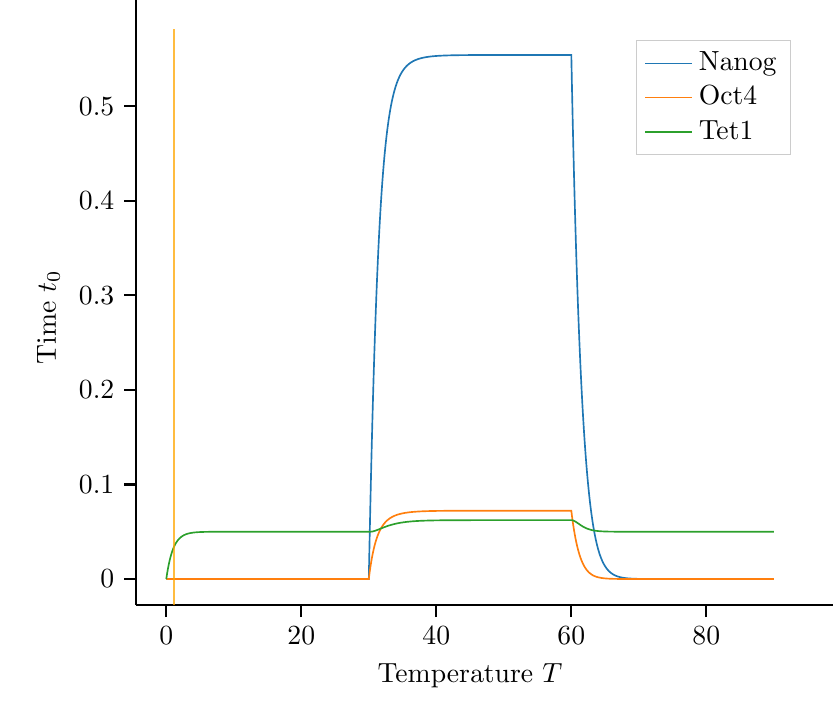
\begin{tikzpicture}

\definecolor{darkgray176}{RGB}{176,176,176}
\definecolor{darkorange25512714}{RGB}{255,127,14}
\definecolor{forestgreen4416044}{RGB}{44,160,44}
\definecolor{lightgray204}{RGB}{204,204,204}
\definecolor{orange}{RGB}{255,165,0}
\definecolor{steelblue31119180}{RGB}{31,119,180}

\begin{axis}[
legend cell align={left},
legend style={fill opacity=0.8, draw opacity=1, text opacity=1, draw=lightgray204},
tick align=outside,
tick pos=left,
x grid style={darkgray176},
xlabel={Temperature \(\displaystyle T\)},
xmin=-4.5, xmax=94.5,
xtick style={color=black},
y grid style={darkgray176},
ylabel={Time \(\displaystyle t_0\)},
ymin=-0.0277047168418057, ymax=0.581799053677921,
ytick style={color=black}
]
\addplot [semithick, steelblue31119180]
table {%
0 0
0.0001 0
0.0011 0
0.0111 0
0.1111 0
0.2111 0
0.3111 0
0.4111 0
0.5111 0
0.6111 0
0.7111 0
0.8111 0
0.9111 0
1.0111 0
1.1111 0
1.2111 0
1.3111 0
1.4111 0
1.5111 0
1.6111 0
1.7111 0
1.8111 0
1.9111 0
2.0111 0
2.1111 0
2.2111 0
2.3111 0
2.4111 0
2.5111 0
2.6111 0
2.7111 0
2.8111 0
2.9111 0
3.0111 0
3.1111 0
3.2111 0
3.3111 0
3.4111 0
3.5111 0
3.6111 0
3.7111 0
3.8111 0
3.9111 0
4.0111 0
4.1111 0
4.2111 0
4.3111 0
4.4111 0
4.5111 0
4.6111 0
4.7111 0
4.8111 0
4.9111 0
5.0111 0
5.1111 0
5.2111 0
5.3111 0
5.4111 0
5.5111 0
5.6111 0
5.7111 0
5.8111 0
5.9111 0
6.0111 0
6.1111 0
6.21109999999999 0
6.31109999999999 0
6.41109999999999 0
6.51109999999999 0
6.61109999999999 0
6.71109999999999 0
6.81109999999999 0
6.91109999999999 0
7.01109999999999 0
7.11109999999999 0
7.21109999999999 0
7.31109999999999 0
7.41109999999999 0
7.51109999999999 0
7.61109999999999 0
7.71109999999999 0
7.81109999999999 0
7.91109999999999 0
8.01109999999999 0
8.11109999999999 0
8.21109999999999 0
8.31109999999999 0
8.41109999999999 0
8.51109999999999 0
8.61109999999999 0
8.71109999999999 0
8.81109999999999 0
8.91109999999999 0
9.01109999999998 0
9.11109999999998 0
9.21109999999998 0
9.31109999999998 0
9.41109999999998 0
9.51109999999998 0
9.61109999999998 0
9.71109999999998 0
9.81109999999998 0
9.91109999999998 0
10.0111 0
10.1111 0
10.2111 0
10.3111 0
10.4111 0
10.5111 0
10.6111 0
10.7111 0
10.8111 0
10.9111 0
11.0111 0
11.1111 0
11.2111 0
11.3111 0
11.4111 0
11.5111 0
11.6111 0
11.7111 0
11.8111 0
11.9111 0
12.0111 0
12.1111 0
12.2111 0
12.3111 0
12.4111 0
12.5111 0
12.6111 0
12.7111 0
12.8111 0
12.9111 0
13.0111 0
13.1111 0
13.2111 0
13.3111 0
13.4111 0
13.5111 0
13.6111 0
13.7111 0
13.8111 0
13.9111 0
14.0111 0
14.1111 0
14.2111 0
14.3111 0
14.4111 0
14.5111 0
14.6111 0
14.7111 0
14.8111 0
14.9111 0
15.0111 0
15.1111 0
15.2111 0
15.3111 0
15.4111 0
15.5111 0
15.6111 0
15.7111 0
15.8111 0
15.9111 0
16.0111 0
16.1111 0
16.2111 0
16.3111 0
16.4111 0
16.5111 0
16.6111 0
16.7111 0
16.8111 0
16.9111 0
17.0111 0
17.1111 0
17.2111 0
17.3111 0
17.4111 0
17.5111 0
17.6111 0
17.7111 0
17.8111 0
17.9111 0
18.0111 0
18.1111 0
18.2111 0
18.3111 0
18.4111 0
18.5111 0
18.6111 0
18.7111 0
18.8111 0
18.9111 0
19.0111 0
19.1111 0
19.2111 0
19.3111 0
19.4111 0
19.5111 0
19.6111 0
19.7111 0
19.8111 0
19.9111 0
20.0111 0
20.1111 0
20.2111 0
20.3111 0
20.4111 0
20.5111 0
20.6111 0
20.7111 0
20.8111 0
20.9111 0
21.0111 0
21.1111 0
21.2111 0
21.3111 0
21.4111 0
21.5111 0
21.6111 0
21.7111 0
21.8111 0
21.9111 0
22.0111 0
22.1111 0
22.2111 0
22.3111 0
22.4111000000001 0
22.5111000000001 0
22.6111000000001 0
22.7111000000001 0
22.8111000000001 0
22.9111000000001 0
23.0111000000001 0
23.1111000000001 0
23.2111000000001 0
23.3111000000001 0
23.4111000000001 0
23.5111000000001 0
23.6111000000001 0
23.7111000000001 0
23.8111000000001 0
23.9111000000001 0
24.0111000000001 0
24.1111000000001 0
24.2111000000001 0
24.3111000000001 0
24.4111000000001 0
24.5111000000001 0
24.6111000000001 0
24.7111000000001 0
24.8111000000001 0
24.9111000000001 0
25.0111000000001 0
25.1111000000001 0
25.2111000000001 0
25.3111000000001 0
25.4111000000001 0
25.5111000000001 0
25.6111000000001 0
25.7111000000001 0
25.8111000000001 0
25.9111000000001 0
26.0111000000001 0
26.1111000000001 0
26.2111000000001 0
26.3111000000001 0
26.4111000000001 0
26.5111000000001 0
26.6111000000001 0
26.7111000000001 0
26.8111000000001 0
26.9111000000001 0
27.0111000000001 0
27.1111000000001 0
27.2111000000001 0
27.3111000000001 0
27.4111000000001 0
27.5111000000001 0
27.6111000000001 0
27.7111000000001 0
27.8111000000001 0
27.9111000000001 0
28.0111000000001 0
28.1111000000001 0
28.2111000000001 0
28.3111000000001 0
28.4111000000001 0
28.5111000000001 0
28.6111000000001 0
28.7111000000001 0
28.8111000000001 0
28.9111000000001 0
29.0111000000001 0
29.1111000000001 0
29.2111000000001 0
29.3111000000001 0
29.4111000000002 0
29.5111000000002 0
29.6111000000002 0
29.7111000000002 0
29.8111000000002 0
29.9111000000002 0
30 0
30 0
30.0026862579625 0.000966475201593659
30.0295488375876 0.010567234068358
30.1295488375876 0.0452583942758918
30.2295488375876 0.0782459863183292
30.3295488375876 0.109500619052527
30.4295488375876 0.139026570208306
30.5295488375876 0.166851792049081
30.6295488375876 0.193020690425914
30.7295488375876 0.217588953979675
30.8295488375876 0.240619799249135
30.9295488375876 0.262181198962019
31.0295488375876 0.282343810375518
31.1295488375876 0.301179415736205
31.2295488375876 0.318759746184408
31.3295488375876 0.335155598007197
31.4295488375876 0.350436174771917
31.5295488375876 0.36466860560323
31.6295488375876 0.377917601627168
31.7295488375876 0.390245221125059
31.8295488375876 0.401710720270754
31.9295488375876 0.41237047112841
32.0295488375876 0.422277932295939
32.1295488375876 0.431483660480442
32.2295488375876 0.440035353586978
32.3295488375876 0.447977917733376
32.4295488375876 0.45535355207523
32.5295488375876 0.462201846513969
32.6295488375876 0.468559888325358
32.7295488375876 0.474462374530762
32.8295488375876 0.479941727473967
32.9295488375876 0.485028211589717
33.0295488375876 0.489750049778177
33.1295488375876 0.494133538149691
33.2295488375876 0.498203158190562
33.3295488375876 0.501981685634416
33.4295488375876 0.505490295514357
33.5295488375876 0.508748663026133
33.6295488375876 0.51177505995804
33.7295488375876 0.514586446544533
33.8295488375876 0.517198558681618
33.9295488375876 0.519625990506542
34.0295488375876 0.521882272395065
34.1295488375876 0.523979944469026
34.2295488375876 0.525930625736958
34.3295488375876 0.527745079012968
34.4295488375876 0.529433271775202
34.5295488375876 0.531004433136221
34.6295488375876 0.532467107104467
34.7295488375876 0.533829202319443
34.8295488375876 0.535098038443998
34.9295488375876 0.536280389395756
35.0295488375876 0.537382523596626
35.1295488375876 0.538410241414986
35.2295488375876 0.539368909969778
35.3295488375876 0.54026349545966
35.4295488375876 0.541098593173781
35.5295488375876 0.541878455333807
35.6295488375876 0.542607016909716
35.7295488375876 0.543287919544664
35.8295488375876 0.543924533717059
35.9295488375876 0.544519979260855
36.0295488375876 0.54507714435817
36.1295488375876 0.545598703111519
36.2295488375876 0.546087131796448
36.3295488375876 0.546544723889063
36.4295488375876 0.546973603956909
36.5295488375876 0.547375740495893
36.6295488375876 0.547752957790511
36.7295488375877 0.5481069468694
36.8295488375877 0.548439275623359
36.9295488375877 0.548751398148331
37.0295488375877 0.549044663371476
37.1295488375877 0.54932032301437
37.2295488375877 0.549579538943474
37.3295488375877 0.549823389954468
37.4295488375877 0.550052878033602
37.5295488375877 0.550268934136091
37.6295488375877 0.550472423518643
37.7295488375877 0.550664150660419
37.8295488375877 0.550844863804205
37.9295488375877 0.551015259147173
38.0295488375877 0.551175984708377
38.1295488375877 0.551327643898112
38.2295488375877 0.551470798812309
38.3295488375877 0.551605973273394
38.4295488375877 0.551733655637378
38.5295488375877 0.551854301385433
38.6295488375877 0.551968335516794
38.7295488375877 0.552076154758519
38.8295488375877 0.552178129606429
38.9295488375877 0.552274606210448
39.0295488375877 0.552365908116507
39.1295488375877 0.552452337876245
39.2295488375877 0.552534178534844
39.3295488375877 0.552611695006528
39.4295488375877 0.552685135346514
39.5295488375877 0.552754731927481
39.6295488375877 0.552820702528038
39.7295488375877 0.552883251340014
39.8295488375877 0.552942569900922
39.9295488375877 0.552998837957391
40.0295488375877 0.553052224264933
40.1295488375877 0.553102887328979
40.2295488375877 0.553150976091724
40.3295488375877 0.553196630568956
40.4295488375877 0.553239982440734
40.5295488375877 0.553281155599452
40.6295488375877 0.55332026665855
40.7295488375877 0.55335742542489
40.8295488375877 0.553392735337559
40.9295488375877 0.553426293875649
41.0295488375877 0.553458192937364
41.1295488375877 0.553488519192621
41.2295488375877 0.553517354411134
41.3295488375877 0.553544775767816
41.4295488375877 0.553570856127204
41.5295488375877 0.553595664308447
41.6295488375877 0.553619265332316
41.7295488375877 0.553641720651544
41.8295488375877 0.553663088365731
41.9295488375877 0.553683423421933
42.0295488375877 0.553702777801989
42.1295488375877 0.553721200697518
42.2295488375877 0.553738738673509
42.3295488375877 0.553755435821292
42.4295488375877 0.553771333901656
42.5295488375877 0.553786472478819
42.6295488375877 0.553800889045876
42.7295488375877 0.553814619142345
42.8295488375877 0.553827696464337
42.9295488375877 0.553840152967876
43.0295488375877 0.553852018965838
43.1295488375877 0.553863323218934
43.2295488375877 0.553874093021158
43.3295488375877 0.553884354280061
43.4295488375877 0.553894131592195
43.5295488375877 0.553903448314066
43.6295488375877 0.553912326628873
43.7295488375877 0.553920787609321
43.8295488375878 0.55392885127676
43.9295488375878 0.553936536656889
44.0295488375878 0.553943861832249
44.1295488375878 0.553950843991701
44.2295488375878 0.553957499477092
44.3295488375878 0.553963843827278
44.4295488375878 0.553969891819667
44.5295488375878 0.553975657509448
44.6295488375878 0.553981154266638
44.7295488375878 0.553986394811079
44.8295488375878 0.553991391245523
44.9295488375878 0.553996155086902
45.0295488375878 0.554000697295908
45.1295488375878 0.554005028304975
45.2295488375878 0.554009158044759
45.3295488375878 0.554013095969202
45.4295488375878 0.55401685107927
45.5295488375878 0.554020431945437
45.6295488375878 0.554023846728976
45.7295488375878 0.554027103202152
45.8295488375878 0.554030208767353
45.9295488375878 0.55403317047523
46.0295488375878 0.554035995041909
46.1295488375878 0.554038688865304
46.2295488375878 0.554041258040612
46.3295488375878 0.554043708375005
46.4295488375878 0.554046045401586
46.5295488375878 0.55404827439263
46.6295488375878 0.554050400372168
46.7295488375878 0.55405242812793
46.8295488375878 0.5540543622227
46.9295488375878 0.554056207005097
47.0295488375878 0.554057966619821
47.1295488375878 0.554059645017402
47.2295488375878 0.554061245963451
47.3295488375878 0.554062773047468
47.4295488375878 0.554064229691215
47.5295488375878 0.554065619156677
47.6295488375878 0.554066944553631
47.7295488375878 0.554068208846857
47.8295488375878 0.554069414862988
47.9295488375878 0.554070565297033
48.0295488375878 0.554071662718582
48.1295488375878 0.554072709577717
48.2295488375878 0.554073708210631
48.3295488375878 0.554074660844981
48.4295488375878 0.554075569604984
48.5295488375878 0.554076436516268
48.6295488375878 0.554077263510495
48.7295488375878 0.554078052429756
48.8295488375878 0.554078805030763
48.9295488375878 0.554079522988837
49.0295488375878 0.554080207901716
49.1295488375878 0.554080861293168
49.2295488375878 0.554081484616443
49.3295488375878 0.554082079257561
49.4295488375878 0.554082646538443
49.5295488375878 0.554083187719891
49.6295488375878 0.554083704004435
49.7295488375878 0.55408419653904
49.8295488375878 0.554084666417687
49.9295488375878 0.554085114683836
50.0295488375878 0.554085542332768
50.1295488375878 0.554085950313824
50.2295488375878 0.554086339532531
50.3295488375878 0.554086710852635
50.4295488375878 0.55408706509804
50.5295488375878 0.554087403054645
50.6295488375878 0.554087725472114
50.7295488375878 0.554088033065546
50.8295488375879 0.554088326517073
50.9295488375879 0.554088606477393
51.0295488375879 0.554088873567214
51.1295488375879 0.554089128378646
51.2295488375879 0.55408937147652
51.3295488375879 0.554089603399649
51.4295488375879 0.554089824662031
51.5295488375879 0.554090035753992
51.6295488375879 0.55409023714328
51.7295488375879 0.554090429276107
51.8295488375879 0.554090612578144
51.9295488375879 0.554090787455466
52.0295488375879 0.554090954295458
52.1295488375879 0.554091113467675
52.2295488375879 0.554091265324668
52.3295488375879 0.554091410202762
52.4295488375879 0.554091548422808
52.5295488375879 0.554091680290895
52.6295488375879 0.55409180609903
52.7295488375879 0.554091926125787
52.8295488375879 0.554092040636927
52.9295488375879 0.554092149885984
53.0295488375879 0.554092254114835
53.1295488375879 0.554092353554228
53.2295488375879 0.554092448424303
53.3295488375879 0.554092538935076
53.4295488375879 0.554092625286902
53.5295488375879 0.554092707670929
53.6295488375879 0.55409278626951
53.7295488375879 0.554092861256619
53.8295488375879 0.554092932798228
53.9295488375879 0.554093001052679
54.0295488375879 0.554093066171035
54.1295488375879 0.554093128297415
54.2295488375879 0.554093187569312
54.3295488375879 0.554093244117899
54.4295488375879 0.55409329806832
54.5295488375879 0.554093349539964
54.6295488375879 0.554093398646736
54.7295488375879 0.554093445497304
54.8295488375879 0.55409349019534
54.9295488375879 0.554093532839753
55.0295488375879 0.554093573524905
55.1295488375879 0.554093612340823
55.2295488375879 0.554093649373394
55.3295488375879 0.55409368470456
55.4295488375879 0.554093718412495
55.5295488375879 0.554093750571784
55.6295488375879 0.55409378125358
55.7295488375879 0.55409381052577
55.8295488375879 0.55409383845312
55.9295488375879 0.554093865097418
56.0295488375879 0.554093890517616
56.1295488375879 0.554093914769956
56.2295488375879 0.554093937908093
56.3295488375879 0.554093959983221
56.4295488375879 0.554093981044177
56.5295488375879 0.554094001137558
56.6295488375879 0.554094020307818
56.7295488375879 0.554094038597367
56.8295488375879 0.55409405604667
56.9295488375879 0.55409407269433
57.0295488375879 0.554094088577176
57.1295488375879 0.554094103730348
57.2295488375879 0.554094118187367
57.3295488375879 0.554094131980217
57.4295488375879 0.554094145139411
57.5295488375879 0.554094157694062
57.6295488375879 0.554094169671943
57.7295488375879 0.554094181099552
57.829548837588 0.55409419200217
57.929548837588 0.554094202403915
58.029548837588 0.5540942123278
58.129548837588 0.554094221795776
58.229548837588 0.55409423082879
58.329548837588 0.554094239446824
58.429548837588 0.554094247668943
58.529548837588 0.554094255513336
58.629548837588 0.554094262997356
58.729548837588 0.554094270137559
58.829548837588 0.554094276949739
58.929548837588 0.554094283448968
59.029548837588 0.554094289649621
59.129548837588 0.554094295565416
59.229548837588 0.554094301209439
59.329548837588 0.554094306594176
59.429548837588 0.554094311731539
59.529548837588 0.554094316632891
59.629548837588 0.554094321309076
59.729548837588 0.554094325770437
59.829548837588 0.554094330026844
59.929548837588 0.554094334087713
60 0.554094336836115
60 0.554094336836115
60.1 0.519217851079352
60.2 0.486485001973495
60.3 0.455750564106413
60.4 0.426881474648157
60.5 0.399755711036345
60.6 0.37426126599693
60.7 0.350295207510073
60.8 0.327762814937749
60.9 0.306576785175355
61 0.286656504496648
61.1 0.267927382875405
61.2 0.250320248141545
61.3 0.2337707975115
61.4 0.218219103955644
61.5 0.20360917464192
61.6 0.189888558413901
61.7 0.17700799898875
61.8 0.164921130340018
61.9 0.153584210586534
62 0.142955890651958
62.1 0.132997013988085
62.2 0.12367044375996
62.3 0.114940914058624
62.4 0.106774901922684
62.5 0.0991405171977778
62.6 0.0920074075294885
62.7 0.0853466760589756
62.8 0.0791308096621312
62.9 0.0733336158358671
63 0.0679301665843949
63.1 0.0628967478912084
63.2 0.0582108135772548
63.3 0.0538509425418023
63.4 0.0497967985596545
63.5 0.0460290919669208
63.6000000000001 0.0425295427080117
63.7000000000001 0.0392808443395541
63.8000000000001 0.0362666286932644
63.9000000000001 0.0334714309903633
64.0000000000001 0.0308806552758349
64.1000000000001 0.0284805401028217
64.2 0.0262581244468899
64.3 0.0242012138680713
64.4 0.0222983469667868
64.5 0.0205387621993324
64.6 0.0189123651308498
64.7 0.0174096962098777
64.8 0.0160218991498454
64.9 0.0147406900003037
65 0.0135583269852367
65.1 0.0124675811782814
65.2 0.0114617080758205
65.3 0.0105344201192662
65.4 0.00967986020791307
65.5 0.00889257623386175
65.6 0.00816749666098815
65.7 0.00749990716096193
65.8 0.00688542831103798
65.8999999999999 0.00631999435084635
65.9999999999999 0.00579983298873171
66.0999999999999 0.00532144624235356
66.1999999999999 0.00488159229323899
66.2999999999999 0.00447726833074671
66.3999999999999 0.0041056943574083
66.4999999999999 0.00376429792480467
66.5999999999999 0.0034506997669534
66.6999999999999 0.00316270029656374
66.7999999999999 0.00289826692839902
66.8999999999999 0.00265552219331097
66.9999999999999 0.00243273260622044
67.0999999999999 0.00222829825135961
67.1999999999999 0.00204074304841363
67.2999999999999 0.00186870566375888
67.3999999999999 0.00171093103174942
67.4999999999999 0.00156626245191697
67.5999999999999 0.00143363422898949
67.6999999999998 0.00131206482377028
67.7999999999998 0.00120065048412955
67.8999999999998 0.00109855932661997
67.9999999999998 0.00100502584051956
68.0999999999998 0.000919345787412942
68.1999999999998 0.000840871470731025
68.2999999999998 0.000769007350969988
68.3999999999998 0.000703205983591837
68.4999999999998 0.000642964257864339
68.5999999999998 0.000587819916121114
68.6999999999998 0.000537348334108354
68.7999999999998 0.000491159544229377
68.8999999999998 0.000448895484599286
68.9999999999998 0.000410227457877469
69.0999999999998 0.00037485378485446
69.1999999999998 0.000342497638731194
69.2999999999998 0.00031290504694286
69.3999999999997 0.000285843048246816
69.4999999999997 0.000261097993615038
69.5999999999997 0.000238473980247348
69.6999999999997 0.000217791408753416
69.7999999999997 0.000198885654240644
69.8999999999997 0.000181605842693
69.9999999999997 0.000165813724634347
70.0999999999997 0.000151382638640394
70.1999999999997 0.000138196557797855
70.2999999999997 0.000126149212709453
70.3999999999997 0.000115143285110699
70.4999999999997 0.000105089666600732
70.5999999999997 9.59067773964878e-05
70.6999999999997 8.75199403987748e-05
70.7999999999997 7.98608062120337e-05
70.8999999999997 7.28668250881882e-05
70.9999999999997 6.64807620705399e-05
71.0999999999997 6.06502518975309e-05
71.1999999999996 5.53273904897645e-05
71.2999999999996 5.04683600882212e-05
71.3999999999996 4.60330853383793e-05
71.4999999999996 4.19849178251042e-05
71.5999999999996 3.82903467578288e-05
71.6999999999996 3.49187336857459e-05
71.7999999999996 3.18420692894731e-05
71.8999999999996 2.90347504498471e-05
71.9999999999996 2.64733759370505e-05
72.0999999999996 2.41365591949789e-05
72.1999999999996 2.20047568174017e-05
72.2999999999996 2.00601114247659e-05
72.3999999999996 1.82863077541366e-05
72.4999999999996 1.66684408703651e-05
72.5999999999996 1.519289549474e-05
72.6999999999996 1.38472355286498e-05
72.7999999999996 1.26201029246711e-05
72.8999999999996 1.15011251264957e-05
72.9999999999995 1.04808303626408e-05
73.0999999999995 9.55057013738404e-06
73.1999999999995 8.70244831620153e-06
73.2999999999995 7.92925625252233e-06
73.3999999999995 7.22441344818025e-06
73.4999999999995 6.58191328184642e-06
73.5999999999995 5.99627337825139e-06
73.6999999999995 5.46249022641584e-06
73.7999999999995 4.97599768764807e-06
73.8999999999995 4.53262906396087e-06
73.9999999999995 4.12858242501802e-06
74.0999999999995 3.76038891693512e-06
74.1999999999995 3.42488379940886e-06
74.2999999999995 3.11917997889781e-06
74.3999999999995 2.84064382507844e-06
74.4999999999995 2.58687307569282e-06
74.5999999999995 2.35567665131852e-06
74.6999999999994 2.14505621664627e-06
74.7999999999994 1.95318933865658e-06
74.8999999999994 1.77841410474486e-06
74.9999999999994 1.61921507544807e-06
75.0999999999994 1.47421045706167e-06
75.1999999999994 1.34214038918191e-06
75.2999999999994 1.22185625113883e-06
75.3999999999994 1.11231089946635e-06
75.4999999999994 1.01254975604987e-06
75.5999999999994 9.21702673454483e-07
75.6999999999994 8.38976510221925e-07
75.7999999999994 7.63648354678151e-07
75.8999999999994 6.95059341061153e-07
75.9999999999994 6.32609006600212e-07
76.0999999999994 5.75750142590524e-07
76.1999999999994 5.23984096545288e-07
76.2999999999994 4.7685648620207e-07
76.3999999999994 4.33953289540561e-07
76.4999999999993 3.94897278060866e-07
76.5999999999993 3.59344763399711e-07
76.6999999999993 3.26982629948383e-07
76.7999999999993 2.97525628501468e-07
76.8999999999993 2.70713908128011e-07
76.9999999999993 2.46310765433875e-07
77.0999999999993 2.24100592191446e-07
77.1999999999993 2.03887003964885e-07
77.2999999999993 1.85491133869006e-07
77.3999999999993 1.6875007697972e-07
77.4999999999993 1.53515472174832e-07
77.5999999999993 1.39652209336023e-07
77.6999999999993 1.27037250895374e-07
77.7999999999993 1.15558557671241e-07
77.8999999999993 1.05114109816585e-07
77.9999999999993 9.56110145049981e-08
78.0999999999993 8.69646927122717e-08
78.1999999999992 7.90981381203524e-08
78.2999999999992 7.19412417814244e-08
78.3999999999992 6.54301767376115e-08
78.4999999999992 5.95068373010239e-08
78.5999999999992 5.41183281637423e-08
78.6999999999992 4.92164989316817e-08
78.7999999999992 4.47575200636062e-08
78.8999999999992 4.0701496550074e-08
78.9999999999992 3.7012115989716e-08
79.0999999999992 3.36563280146612e-08
79.1999999999992 3.06040522855689e-08
79.2999999999992 2.78279125218503e-08
79.3999999999992 2.53029942562993e-08
79.4999999999992 2.30066242073814e-08
79.5999999999992 2.09181693485511e-08
79.6999999999992 1.90188539237415e-08
79.7999999999992 1.72915928130326e-08
79.8999999999992 1.57208397937375e-08
79.9999999999991 1.42924493709623e-08
80.0999999999991 1.29935509691617e-08
80.1999999999991 1.18124343833328e-08
80.2999999999991 1.07384454861649e-08
80.3999999999991 9.76189127652446e-09
80.4999999999991 8.8739534358505e-09
80.5999999999991 8.06660963306426e-09
80.6999999999991 7.33256188608224e-09
80.7999999999991 6.66517134953927e-09
80.8999999999991 6.05839895440463e-09
80.9999999999991 5.50675137628546e-09
81.0999999999991 5.00523185579699e-09
81.1999999999991 4.54929543683582e-09
81.2999999999991 4.13480822728451e-09
81.3999999999991 3.75801032193637e-09
81.4999999999991 3.41548205955927e-09
81.5999999999991 3.1041133152949e-09
81.6999999999991 2.82107555626595e-09
81.799999999999 2.56379641256879e-09
81.899999999999 2.32993653797245e-09
81.999999999999 2.1173685548183e-09
82.099999999999 1.92415789599208e-09
82.199999999999 1.74854537358092e-09
82.299999999999 1.58893131907733e-09
82.399999999999 1.44386115388196e-09
82.499999999999 1.31201226150825e-09
82.599999999999 1.1921820444148e-09
82.699999999999 1.08327705888506e-09
82.799999999999 9.84303130931234e-10
82.899999999999 8.94356364902453e-10
82.999999999999 8.12614964402606e-10
83.099999999999 7.38331792340216e-10
83.199999999999 6.70827603504004e-10
83.299999999999 6.09484889041153e-10
83.399999999999 5.53742277663019e-10
83.4999999999989 5.03089443362949e-10
83.5999999999989 4.57062473946415e-10
83.6999999999989 4.15239658784578e-10
83.7999999999989 3.77237657944704e-10
83.8999999999989 3.42708018257597e-10
83.9999999999989 3.11334004983224e-10
84.0999999999989 2.82827720558462e-10
84.1999999999989 2.56927484480199e-10
84.2999999999989 2.3339545071552e-10
84.3999999999989 2.12015441159182e-10
84.4999999999989 1.92590975595661e-10
84.5999999999989 1.74943480386038e-10
84.6999999999989 1.589106597044e-10
84.7999999999989 1.44345014608464e-10
84.8999999999989 1.31112496557799e-10
84.9999999999989 1.19091283202075e-10
85.0999999999989 1.0817066536188e-10
85.1999999999989 9.82500351257375e-11
85.2999999999988 8.92379658977732e-11
85.3999999999988 8.1051376059212e-11
85.4999999999988 7.36147686609086e-11
85.5999999999988 6.68595402501011e-11
85.6999999999988 6.07233525586874e-11
85.7999999999988 5.51495613481017e-11
85.8999999999988 5.00866972223921e-11
85.9999999999988 4.54879936909748e-11
86.0999999999988 4.13109581899772e-11
86.1999999999988 3.75169821598928e-11
86.2999999999988 3.40709866309458e-11
86.3999999999988 3.0941100089257e-11
86.4999999999988 2.80983656895137e-11
86.5999999999988 2.55164751459815e-11
86.6999999999988 2.31715268757559e-11
86.7999999999988 2.10418061883042e-11
86.8999999999988 1.91075855155669e-11
86.9999999999987 1.73509428589831e-11
87.0999999999987 1.57555967953981e-11
87.1999999999987 1.43067565344122e-11
87.2999999999987 1.2990985656674e-11
87.3999999999987 1.17960782871587e-11
87.4999999999987 1.07109465707161e-11
87.5999999999987 9.72551842014575e-12
87.6999999999987 8.83064460069138e-12
87.7999999999987 8.01801429998405e-12
87.8999999999987 7.28007840987436e-12
87.9999999999987 6.60997981697905e-12
88.0999999999987 6.00149006276056e-12
88.1999999999987 5.44895179214017e-12
88.2999999999987 4.94722646254212e-12
88.3999999999987 4.49164683335703e-12
88.4999999999987 4.07797379953295e-12
88.5999999999987 3.70235717274883e-12
88.6999999999987 3.36130004975745e-12
88.7999999999986 3.05162644033173e-12
88.8999999999986 2.77045185710714e-12
88.9999999999986 2.51515659675553e-12
89.0999999999986 2.2833614665981e-12
89.1999999999986 2.07290573319265e-12
89.2999999999986 1.8818270898149e-12
89.3999999999986 1.70834345828367e-12
89.4999999999986 1.55083645742066e-12
89.5999999999986 1.40783638574368e-12
89.6999999999986 1.27800857990468e-12
89.7999999999986 1.16014102302948e-12
89.8999999999986 1.05313308860792e-12
89.9999999999986 9.55985316028894e-13
90 9.5598531602758e-13
};
\addlegendentry{Nanog}
\addplot [semithick, darkorange25512714]
table {%
0 0
0.0001 0
0.0011 0
0.0111 0
0.1111 0
0.2111 0
0.3111 0
0.4111 0
0.5111 0
0.6111 0
0.7111 0
0.8111 0
0.9111 0
1.0111 0
1.1111 0
1.2111 0
1.3111 0
1.4111 0
1.5111 0
1.6111 0
1.7111 0
1.8111 0
1.9111 0
2.0111 0
2.1111 0
2.2111 0
2.3111 0
2.4111 0
2.5111 0
2.6111 0
2.7111 0
2.8111 0
2.9111 0
3.0111 0
3.1111 0
3.2111 0
3.3111 0
3.4111 0
3.5111 0
3.6111 0
3.7111 0
3.8111 0
3.9111 0
4.0111 0
4.1111 0
4.2111 0
4.3111 0
4.4111 0
4.5111 0
4.6111 0
4.7111 0
4.8111 0
4.9111 0
5.0111 0
5.1111 0
5.2111 0
5.3111 0
5.4111 0
5.5111 0
5.6111 0
5.7111 0
5.8111 0
5.9111 0
6.0111 0
6.1111 0
6.21109999999999 0
6.31109999999999 0
6.41109999999999 0
6.51109999999999 0
6.61109999999999 0
6.71109999999999 0
6.81109999999999 0
6.91109999999999 0
7.01109999999999 0
7.11109999999999 0
7.21109999999999 0
7.31109999999999 0
7.41109999999999 0
7.51109999999999 0
7.61109999999999 0
7.71109999999999 0
7.81109999999999 0
7.91109999999999 0
8.01109999999999 0
8.11109999999999 0
8.21109999999999 0
8.31109999999999 0
8.41109999999999 0
8.51109999999999 0
8.61109999999999 0
8.71109999999999 0
8.81109999999999 0
8.91109999999999 0
9.01109999999998 0
9.11109999999998 0
9.21109999999998 0
9.31109999999998 0
9.41109999999998 0
9.51109999999998 0
9.61109999999998 0
9.71109999999998 0
9.81109999999998 0
9.91109999999998 0
10.0111 0
10.1111 0
10.2111 0
10.3111 0
10.4111 0
10.5111 0
10.6111 0
10.7111 0
10.8111 0
10.9111 0
11.0111 0
11.1111 0
11.2111 0
11.3111 0
11.4111 0
11.5111 0
11.6111 0
11.7111 0
11.8111 0
11.9111 0
12.0111 0
12.1111 0
12.2111 0
12.3111 0
12.4111 0
12.5111 0
12.6111 0
12.7111 0
12.8111 0
12.9111 0
13.0111 0
13.1111 0
13.2111 0
13.3111 0
13.4111 0
13.5111 0
13.6111 0
13.7111 0
13.8111 0
13.9111 0
14.0111 0
14.1111 0
14.2111 0
14.3111 0
14.4111 0
14.5111 0
14.6111 0
14.7111 0
14.8111 0
14.9111 0
15.0111 0
15.1111 0
15.2111 0
15.3111 0
15.4111 0
15.5111 0
15.6111 0
15.7111 0
15.8111 0
15.9111 0
16.0111 0
16.1111 0
16.2111 0
16.3111 0
16.4111 0
16.5111 0
16.6111 0
16.7111 0
16.8111 0
16.9111 0
17.0111 0
17.1111 0
17.2111 0
17.3111 0
17.4111 0
17.5111 0
17.6111 0
17.7111 0
17.8111 0
17.9111 0
18.0111 0
18.1111 0
18.2111 0
18.3111 0
18.4111 0
18.5111 0
18.6111 0
18.7111 0
18.8111 0
18.9111 0
19.0111 0
19.1111 0
19.2111 0
19.3111 0
19.4111 0
19.5111 0
19.6111 0
19.7111 0
19.8111 0
19.9111 0
20.0111 0
20.1111 0
20.2111 0
20.3111 0
20.4111 0
20.5111 0
20.6111 0
20.7111 0
20.8111 0
20.9111 0
21.0111 0
21.1111 0
21.2111 0
21.3111 0
21.4111 0
21.5111 0
21.6111 0
21.7111 0
21.8111 0
21.9111 0
22.0111 0
22.1111 0
22.2111 0
22.3111 0
22.4111000000001 0
22.5111000000001 0
22.6111000000001 0
22.7111000000001 0
22.8111000000001 0
22.9111000000001 0
23.0111000000001 0
23.1111000000001 0
23.2111000000001 0
23.3111000000001 0
23.4111000000001 0
23.5111000000001 0
23.6111000000001 0
23.7111000000001 0
23.8111000000001 0
23.9111000000001 0
24.0111000000001 0
24.1111000000001 0
24.2111000000001 0
24.3111000000001 0
24.4111000000001 0
24.5111000000001 0
24.6111000000001 0
24.7111000000001 0
24.8111000000001 0
24.9111000000001 0
25.0111000000001 0
25.1111000000001 0
25.2111000000001 0
25.3111000000001 0
25.4111000000001 0
25.5111000000001 0
25.6111000000001 0
25.7111000000001 0
25.8111000000001 0
25.9111000000001 0
26.0111000000001 0
26.1111000000001 0
26.2111000000001 0
26.3111000000001 0
26.4111000000001 0
26.5111000000001 0
26.6111000000001 0
26.7111000000001 0
26.8111000000001 0
26.9111000000001 0
27.0111000000001 0
27.1111000000001 0
27.2111000000001 0
27.3111000000001 0
27.4111000000001 0
27.5111000000001 0
27.6111000000001 0
27.7111000000001 0
27.8111000000001 0
27.9111000000001 0
28.0111000000001 0
28.1111000000001 0
28.2111000000001 0
28.3111000000001 0
28.4111000000001 0
28.5111000000001 0
28.6111000000001 0
28.7111000000001 0
28.8111000000001 0
28.9111000000001 0
29.0111000000001 0
29.1111000000001 0
29.2111000000001 0
29.3111000000001 0
29.4111000000002 0
29.5111000000002 0
29.6111000000002 0
29.7111000000002 0
29.8111000000002 0
29.9111000000002 0
30 0
30 0
30.0026862579625 0.000160959192932928
30.0295488375876 0.00174700466258397
30.1295488375876 0.00729368481827424
30.2295488375876 0.0123289305767425
30.3295488375876 0.0169149747621551
30.4295488375876 0.021102923870268
30.5295488375876 0.0249346852800907
30.6295488375876 0.0284454622466816
30.7295488375876 0.031665564913883
30.8295488375876 0.0346215909725772
30.9295488375876 0.037337190862689
31.0295488375876 0.0398335800903369
31.1295488375876 0.0421298993857418
31.2295488375876 0.0442434817931022
31.3295488375876 0.0461900610086228
31.4295488375876 0.0479839410552
31.5295488375876 0.0496381392574179
31.6295488375876 0.0511645098105133
31.7295488375876 0.0525738525208938
31.8295488375876 0.0538760096931989
31.9295488375876 0.0550799531778107
32.0295488375876 0.0561938630057026
32.1295488375876 0.0572251986712339
32.2295488375876 0.0581807638890017
32.3295488375876 0.059066765495964
32.4295488375876 0.0598888670637878
32.5295488375876 0.0606522377102389
32.6295488375876 0.0613615965412508
32.7295488375876 0.0620212531102943
32.8295488375876 0.0626351442446891
32.9295488375876 0.0632068675569978
33.0295488375876 0.0637397119320619
33.1295488375876 0.0642366852555844
33.2295488375876 0.064700539627836
33.3295488375876 0.0651337942856456
33.4295488375876 0.0655387564370789
33.5295488375876 0.0659175401959299
33.6295488375876 0.0662720837872018
33.7295488375876 0.0666041651800496
33.8295488375876 0.066915416291093
33.9295488375876 0.0672073358885153
34.0295488375876 0.0674813013158713
34.1295488375876 0.0677385791439666
34.2295488375876 0.0679803348494756
34.3295488375876 0.068207641610087
34.4295488375876 0.0684214882978304
34.5295488375876 0.0686227867448049
34.6295488375876 0.0688123783487389
34.7295488375876 0.0689910400796149
34.8295488375876 0.0691594899429424
34.9295488375876 0.0693183919501205
35.0295488375876 0.0694683606416448
35.1295488375876 0.0696099652046581
35.2295488375876 0.0697437332224686
35.3295488375876 0.0698701540901474
35.4295488375876 0.0699896821271197
35.5295488375876 0.0701027394147685
35.6295488375876 0.0702097183844404
35.7295488375876 0.0703109841788579
35.8295488375876 0.0704068768077836
35.9295488375876 0.0704977131168207
36.0295488375876 0.0705837885864629
36.1295488375876 0.0706653789768947
36.2295488375876 0.070742741832593
36.3295488375876 0.0708161178594578
36.4295488375876 0.0708857321860097
36.5295488375876 0.0709517955191088
36.6295488375876 0.0710145052036743
36.7295488375877 0.0710740461949957
36.8295488375877 0.0711305919514291
36.9295488375877 0.0711843052545419
37.0295488375877 0.0712353389631178
37.1295488375877 0.0712838367068365
37.2295488375877 0.0713299335249054
37.3295488375877 0.0713737564544351
37.4295488375877 0.0714154250729072
37.5295488375877 0.0714550519986872
37.6295488375877 0.0714927433531707
37.7295488375877 0.0715285991878258
37.8295488375877 0.0715627138790984
37.9295488375877 0.0715951764938777
38.0295488375877 0.0716260711279756
38.1295488375877 0.0716554772198559
38.2295488375877 0.0716834698416462
38.3295488375877 0.0717101199692853
38.4295488375877 0.0717354947334975
38.5295488375877 0.0717596576531312
38.6295488375877 0.0717826688522684
38.7295488375877 0.0718045852623867
38.8295488375877 0.0718254608107456
38.9295488375877 0.0718453465960659
39.0295488375877 0.0718642910524821
39.1295488375877 0.0718823401026602
39.2295488375877 0.0718995373009021
39.3295488375877 0.071915923966985
39.4295488375877 0.0719315393114241
39.5295488375877 0.0719464205527877
39.6295488375877 0.0719606030276439
39.7295488375877 0.071974120293669
39.8295488375877 0.0719870042264061
39.9295488375877 0.0719992851101215
40.0295488375877 0.0720109917231721
40.1295488375877 0.0720221514182635
40.2295488375877 0.0720327901979485
40.3295488375877 0.0720429327856893
40.4295488375877 0.0720526026927803
40.5295488375877 0.0720618222814073
40.6295488375877 0.0720706128240962
40.7295488375877 0.0720789945597879
40.8295488375877 0.0720869867467537
40.9295488375877 0.0720946077125567
41.0295488375877 0.0721018749012421
41.1295488375877 0.0721088049179318
41.2295488375877 0.0721154135709838
41.3295488375877 0.0721217159118643
41.4295488375877 0.0721277262728735
41.5295488375877 0.0721334583028526
41.6295488375877 0.072138925000993
41.7295488375877 0.0721441387488595
41.8295488375877 0.0721491113407325
41.9295488375877 0.0721538540123664
42.0295488375877 0.0721583774682552
42.1295488375877 0.0721626919074905
42.2295488375877 0.0721668070482921
42.3295488375877 0.0721707321512845
42.4295488375877 0.0721744760415906
42.5295488375877 0.0721780471298066
42.6295488375877 0.0721814534319205
42.7295488375877 0.0721847025882308
42.8295488375877 0.0721878018813207
42.9295488375877 0.0721907582531368
43.0295488375877 0.0721935783212219
43.1295488375877 0.0721962683941455
43.2295488375877 0.0721988344861749
43.3295488375877 0.072201282331226
43.4295488375877 0.0722036173961322
43.5295488375877 0.0722058448932665
43.6295488375877 0.0722079697925488
43.7295488375877 0.0722099968328727
43.8295488375878 0.072211930532978
43.9295488375878 0.0722137752017998
44.0295488375878 0.0722155349483192
44.1295488375878 0.0722172136909416
44.2295488375878 0.0722188151664246
44.3295488375878 0.0722203429383802
44.4295488375878 0.072221800405371
44.5295488375878 0.0722231908086204
44.6295488375878 0.0722245172393569
44.7295488375878 0.0722257826458097
44.8295488375878 0.0722269898398724
44.9295488375878 0.0722281415034524
45.0295488375878 0.0722292401945198
45.1295488375878 0.0722302883528705
45.2295488375878 0.0722312883056193
45.3295488375878 0.0722322422724327
45.4295488375878 0.0722331523705179
45.5295488375878 0.0722340206193754
45.6295488375878 0.0722348489453309
45.7295488375878 0.0722356391858533
45.8295488375878 0.0722363930936717
45.9295488375878 0.0722371123406997
46.0295488375878 0.0722377985217759
46.1295488375878 0.0722384531582307
46.2295488375878 0.0722390777012862
46.3295488375878 0.0722396735352977
46.4295488375878 0.072240241980845
46.5295488375878 0.0722407842976786
46.6295488375878 0.0722413016875303
46.7295488375878 0.0722417952967922
46.8295488375878 0.0722422662190715
46.9295488375878 0.0722427154976275
47.0295488375878 0.072243144127694
47.1295488375878 0.072243553058696
47.2295488375878 0.0722439431963615
47.3295488375878 0.0722443154047374
47.4295488375878 0.0722446705081109
47.5295488375878 0.0722450092928425
47.6295488375878 0.0722453325091136
47.7295488375878 0.0722456408725942
47.8295488375878 0.0722459350660326
47.9295488375878 0.0722462157407722
48.0295488375878 0.072246483518198
48.1295488375878 0.0722467389911161
48.2295488375878 0.07224698272507
48.3295488375878 0.0722472152595957
48.4295488375878 0.0722474371094191
48.5295488375878 0.0722476487655979
48.6295488375878 0.072247850696611
48.7295488375878 0.0722480433493979
48.8295488375878 0.0722482271503496
48.9295488375878 0.0722484025062543
49.0295488375878 0.0722485698051994
49.1295488375878 0.0722487294174316
49.2295488375878 0.0722488816961778
49.3295488375878 0.0722490269784283
49.4295488375878 0.072249165585683
49.5295488375878 0.0722492978246643
49.6295488375878 0.0722494239879968
49.7295488375878 0.0722495443548553
49.8295488375878 0.0722496591915837
49.9295488375878 0.0722497687522845
50.0295488375878 0.0722498732793824
50.1295488375878 0.0722499730041604
50.2295488375878 0.0722500681472727
50.3295488375878 0.0722501589192331
50.4295488375878 0.0722502455208812
50.5295488375878 0.0722503281438273
50.6295488375878 0.0722504069708763
50.7295488375878 0.072250482176433
50.8295488375879 0.0722505539268876
50.9295488375879 0.0722506223809848
51.0295488375879 0.0722506876901745
51.1295488375879 0.0722507499989477
51.2295488375879 0.072250809445156
51.3295488375879 0.0722508661603168
51.4295488375879 0.0722509202699045
51.5295488375879 0.0722509718936281
51.6295488375879 0.0722510211456963
51.7295488375879 0.0722510681350703
51.8295488375879 0.0722511129657047
51.9295488375879 0.0722511557367779
52.0295488375879 0.0722511965429112
52.1295488375879 0.0722512354743789
52.2295488375879 0.072251272617307
52.3295488375879 0.072251308053865
52.4295488375879 0.0722513418624467
52.5295488375879 0.0722513741178443
52.6295488375879 0.0722514048914137
52.7295488375879 0.0722514342512326
52.8295488375879 0.0722514622622506
52.9295488375879 0.0722514889864335
53.0295488375879 0.0722515144829002
53.1295488375879 0.0722515388080534
53.2295488375879 0.0722515620157045
53.3295488375879 0.0722515841571926
53.4295488375879 0.0722516052814983
53.5295488375879 0.0722516254353518
53.6295488375879 0.0722516446633364
53.7295488375879 0.0722516630079872
53.8295488375879 0.0722516805098851
53.9295488375879 0.0722516972077467
54.0295488375879 0.0722517131385097
54.1295488375879 0.0722517283374151
54.2295488375879 0.0722517428380847
54.3295488375879 0.0722517566725957
54.4295488375879 0.0722517698715516
54.5295488375879 0.0722517824641501
54.6295488375879 0.0722517944782472
54.7295488375879 0.0722518059404195
54.8295488375879 0.0722518168760224
54.9295488375879 0.0722518273092467
55.0295488375879 0.0722518372631716
55.1295488375879 0.0722518467598161
55.2295488375879 0.0722518558201878
55.3295488375879 0.0722518644643289
55.4295488375879 0.0722518727113612
55.5295488375879 0.0722518805795277
55.6295488375879 0.0722518880862335
55.7295488375879 0.072251895248084
55.8295488375879 0.0722519020809219
55.9295488375879 0.0722519085998619
56.0295488375879 0.0722519148193245
56.1295488375879 0.0722519207530675
56.2295488375879 0.0722519264142169
56.3295488375879 0.0722519318152956
56.4295488375879 0.0722519369682511
56.5295488375879 0.0722519418844821
56.6295488375879 0.0722519465748637
56.7295488375879 0.0722519510497713
56.8295488375879 0.0722519553191038
56.9295488375879 0.0722519593923051
57.0295488375879 0.0722519632783856
57.1295488375879 0.0722519669859414
57.2295488375879 0.0722519705231739
57.3295488375879 0.0722519738979077
57.4295488375879 0.0722519771176079
57.5295488375879 0.0722519801893967
57.6295488375879 0.0722519831200691
57.7295488375879 0.0722519859161079
57.829548837588 0.0722519885836982
57.929548837588 0.0722519911287407
58.029548837588 0.0722519935568653
58.129548837588 0.0722519958734432
58.229548837588 0.0722519980835987
58.329548837588 0.0722520001922208
58.429548837588 0.072252002203974
58.529548837588 0.0722520041233083
58.629548837588 0.0722520059544694
58.729548837588 0.072252007701508
58.829548837588 0.0722520093682886
58.929548837588 0.0722520109584982
59.029548837588 0.0722520124756544
59.129548837588 0.0722520139231134
59.229548837588 0.0722520153040768
59.329548837588 0.0722520166215996
59.429548837588 0.0722520178785961
59.529548837588 0.0722520190778469
59.629548837588 0.0722520202220048
59.729548837588 0.0722520213136007
59.829548837588 0.0722520223550494
59.929548837588 0.0722520233486544
60 0.0722520240211281
60 0.0722520240211281
60.1 0.0664900786004402
60.2 0.0611760249780536
60.3 0.0562713251192646
60.4 0.0517419053285664
60.5 0.0475575042284112
60.6 0.0436911076937085
60.7 0.0401184645051677
60.8 0.0368176755685557
60.9 0.0337688490081555
61 0.0309538132482681
61.1 0.0283558803008975
61.2 0.0259596518261944
61.3 0.0237508610656505
61.4 0.0217162444072296
61.5 0.0198434370713938
61.6 0.0181208881592448
61.7 0.0165377910396618
61.8 0.0150840257420515
61.9 0.0137501106453279
62 0.0125271613007912
62.1 0.011406854692636
62.2 0.010381397626506
62.3 0.0094434982494964
62.4 0.00858633995258519
62.5 0.00780355709833167
62.6 0.00708921216282201
62.7 0.00643777399082768
62.8 0.00584409694551049
62.9 0.00530340079592783
63 0.00481125123273403
63.1 0.00436354093903656
63.2 0.00395647117224249
63.3 0.00358653383575949
63.4 0.00325049403766381
63.5 0.00294537314749294
63.6000000000001 0.00266843237248302
63.7000000000001 0.00241715688109713
63.8000000000001 0.00218924050485989
63.9000000000001 0.00198257104969475
64.0000000000001 0.00179521624561641
64.1000000000001 0.00162541035929384
64.2 0.00147154148823348
64.3 0.00133213954868821
64.4 0.00120586496237826
64.5 0.00109149804014532
64.6 0.000987929054089359
64.7 0.000894148983807204
64.8 0.000809240917222691
64.9 0.000732372082252753
65 0.000662786482211293
65.1 0.000599798105384146
65.2 0.000542784677549465
65.3 0.000491181925282703
65.4 0.000444478317576251
65.5 0.000402210253519747
65.6 0.000363957664429429
65.7 0.000329339999791982
65.8 0.000298012567617087
65.8999999999999 0.000269663201201206
65.9999999999999 0.000244009225831144
66.0999999999999 0.000220794700548469
66.1999999999999 0.00019978791171326
66.2999999999999 0.000180779096714943
66.3999999999999 0.000163578377753761
66.4999999999999 0.000148013887139884
66.5999999999999 0.000133930067014684
66.6999999999999 0.00012118612778134
66.7999999999999 0.000109654650834207
66.8999999999999 9.92203223956067e-05
66.9999999999999 8.97787864045127e-05
67.0999999999999 8.12356054550941e-05
67.1999999999999 7.35053197568219e-05
67.2999999999999 6.65105949849402e-05
67.3999999999999 6.0181450714526e-05
67.4999999999999 5.44545618872266e-05
67.5999999999999 4.92726264514578e-05
67.6999999999998 4.45837929487687e-05
67.7999999999998 4.03411423955791e-05
67.8999999999998 3.65022193347984e-05
67.9999999999998 3.30286074099902e-05
68.0999999999998 2.98855452496036e-05
68.1999999999998 2.7041578843969e-05
68.2999999999998 2.44682469566445e-05
68.3999999999998 2.2139796437448e-05
68.4999999999998 2.00329246000446e-05
68.5999999999998 1.81265460949673e-05
68.6999999999998 1.64015819519216e-05
68.7999999999998 1.48407686854261e-05
68.8999999999998 1.34284855573611e-05
68.9999999999998 1.21505982707418e-05
69.0999999999998 1.09943175327359e-05
69.1999999999998 9.94807107318943e-06
69.2999999999998 9.00138783916221e-06
69.3999999999997 8.14479320750223e-06
69.4999999999997 7.36971416750953e-06
69.5999999999997 6.66839352533267e-06
69.6999999999997 6.03381227188727e-06
69.7999999999997 5.45961933767864e-06
69.8999999999997 4.94006803175643e-06
69.9999999999997 4.4699585288628e-06
70.0999999999997 4.04458582931874e-06
70.1999999999997 3.65969267092953e-06
70.2999999999997 3.31142692172371e-06
70.3999999999997 2.99630302716427e-06
70.4999999999997 2.71116712603321e-06
70.5999999999997 2.45316548589575e-06
70.6999999999997 2.21971594226447e-06
70.7999999999997 2.00848205563903e-06
70.8999999999997 1.81734972779271e-06
70.9999999999997 1.64440604328653e-06
71.0999999999997 1.48792012445891e-06
71.1999999999996 1.34632580828854e-06
71.2999999999996 1.21820597175997e-06
71.3999999999996 1.10227834885906e-06
71.4999999999996 9.9738269725307e-07
71.5999999999996 9.02469186217609e-07
71.6999999999996 8.16587889594593e-07
71.7999999999996 7.38879278624599e-07
71.8999999999996 6.68565619503669e-07
71.9999999999996 6.04943189569185e-07
72.0999999999996 5.47375234212361e-07
72.1999999999996 4.9528559402819e-07
72.2999999999996 4.4815293842156e-07
72.3999999999996 4.0550554795777e-07
72.4999999999996 3.66916593237641e-07
72.5999999999996 3.31999863046761e-07
72.6999999999996 3.00405899024848e-07
72.7999999999996 2.7181849816979e-07
72.8999999999996 2.45951548172297e-07
72.9999999999995 2.22546163908181e-07
73.0999999999995 2.01368096429355e-07
73.1999999999995 1.82205388521878e-07
73.2999999999995 1.64866253367107e-07
73.3999999999995 1.49177155074907e-07
73.4999999999995 1.34981071878242e-07
73.5999999999995 1.22135924606645e-07
73.6999999999995 1.10513154710188e-07
73.7999999999995 9.99964376023597e-08
73.8999999999995 9.04805184445421e-08
73.9999999999995 8.18701587202421e-08
74.0999999999995 7.4079183056031e-08
74.1999999999995 6.70296167494623e-08
74.2999999999995 6.06509053720574e-08
74.3999999999995 5.48792086368829e-08
74.4999999999995 4.96567614635121e-08
74.5999999999995 4.49312958456926e-08
74.6999999999994 4.06555177355784e-08
74.7999999999994 3.6786633709009e-08
74.8999999999994 3.3285922674541e-08
74.9999999999994 3.01183483397553e-08
75.0999999999994 2.72522085562687e-08
75.1999999999994 2.46588180339811e-08
75.2999999999994 2.2312221249053e-08
75.3999999999994 2.01889326723008e-08
75.4999999999994 1.82677017181293e-08
75.5999999999994 1.65293000615299e-08
75.6999999999994 1.49563291945426e-08
75.7999999999994 1.35330462961415e-08
75.8999999999994 1.22452066727922e-08
75.9999999999994 1.1079921192772e-08
76.0999999999994 1.0025527287408e-08
76.1999999999994 9.07147222817127e-09
76.2999999999994 8.20820751142297e-09
76.3999999999994 7.4270932937817e-09
76.4999999999993 6.72031192166735e-09
76.5999999999993 6.08078968959705e-09
76.6999999999993 5.50212604416357e-09
76.7999999999993 4.97852952514604e-09
76.8999999999993 4.50475980262978e-09
76.9999999999993 4.07607523002358e-09
77.0999999999993 3.6881853880672e-09
77.1999999999993 3.33720814487361e-09
77.2999999999993 3.01963080224853e-09
77.3999999999993 2.73227493942647e-09
77.4999999999993 2.47226460236758e-09
77.5999999999993 2.23699752024322e-09
77.6999999999993 2.02411906103499e-09
77.7999999999993 1.83149866558623e-09
77.8999999999993 1.65720852425002e-09
77.9999999999993 1.4995042827224e-09
78.0999999999993 1.35680758395833e-09
78.1999999999992 1.22769027144396e-09
78.2999999999992 1.11086009572631e-09
78.3999999999992 1.00514778114653e-09
78.4999999999992 9.09495323336111e-10
78.5999999999992 8.22945400353694e-10
78.6999999999992 7.44631791485334e-10
78.7999999999992 6.7377070781652e-10
78.8999999999992 6.09652947809327e-10
78.9999999999992 5.51636799375101e-10
79.0999999999992 4.99141617404233e-10
79.1999999999992 4.51642012474774e-10
79.2999999999992 4.08662592578548e-10
79.3999999999992 3.69773205238183e-10
79.4999999999992 3.34584632396561e-10
79.5999999999992 3.02744694991713e-10
79.6999999999992 2.73934728230416e-10
79.7999999999992 2.47866392283855e-10
79.8999999999992 2.24278786485721e-10
79.9999999999991 2.02935838150674e-10
80.0999999999991 1.83623939879568e-10
80.1999999999991 1.66149811704825e-10
80.2999999999991 1.50338566679564e-10
80.3999999999991 1.36031960550271e-10
80.4999999999991 1.2308680799513e-10
80.5999999999991 1.11373549577205e-10
80.6999999999991 1.00774955070058e-10
80.7999999999991 9.11849501782495e-11
80.8999999999991 8.25075549101413e-11
80.9999999999991 7.46559229778884e-11
81.0999999999991 6.75514726106051e-11
81.1999999999991 6.11231000815952e-11
81.2999999999991 5.53064680783608e-11
81.3999999999991 5.00433617931592e-11
81.4999999999991 4.52811062896434e-11
81.5999999999991 4.09720393143984e-11
81.6999999999991 3.70730342770923e-11
81.799999999999 3.35450686250676e-11
81.899999999999 3.03528332925208e-11
81.999999999999 2.74643793155068e-11
82.099999999999 2.48507980759707e-11
82.199999999999 2.24859319745844e-11
82.299999999999 2.0346112636702e-11
82.399999999999 1.84099240313128e-11
82.499999999999 1.66579881322059e-11
82.599999999999 1.50727709761726e-11
82.699999999999 1.36384071772097e-11
82.799999999999 1.23405411404053e-11
82.899999999999 1.11661833863207e-11
82.999999999999 1.0103580547915e-11
83.099999999999 9.14209773889836e-12
83.199999999999 8.27211211621585e-12
83.299999999999 7.48491657140068e-12
83.399999999999 6.77263258690661e-12
83.4999999999989 6.12813138525682e-12
83.5999999999989 5.54496258184329e-12
83.6999999999989 5.01728962731004e-12
83.7999999999989 4.53983139340586e-12
83.8999999999989 4.107809317678e-12
83.9999999999989 3.71689957801339e-12
84.0999999999989 3.36318981837391e-12
84.1999999999989 3.04313999262242e-12
84.2999999999989 2.7535469345514e-12
84.3999999999989 2.49151229951917e-12
84.4999999999989 2.25441355684269e-12
84.5999999999989 2.03987774262922e-12
84.6999999999989 1.84575771035626e-12
84.7999999999989 1.67011064150761e-12
84.8999999999989 1.51117860119278e-12
84.9999999999989 1.36737094414386e-12
85.0999999999989 1.23724839500315e-12
85.1999999999989 1.11950864357172e-12
85.2999999999988 1.01297331085129e-12
85.3999999999988 9.16576155431257e-13
85.4999999999988 8.29352402186315e-13
85.5999999999988 7.50429086482818e-13
85.6999999999988 6.79016317255358e-13
85.7999999999988 6.1439937151155e-13
85.8999999999988 5.55931541144136e-13
85.9999999999988 5.03027660458934e-13
86.0999999999988 4.55158249639921e-13
86.1999999999988 4.11844215537308e-13
86.2999999999988 3.72652056742297e-13
86.3999999999988 3.37189524959308e-13
86.4999999999988 3.05101699253225e-13
86.5999999999988 2.76067433881403e-13
86.6999999999988 2.49796144159158e-13
86.7999999999988 2.26024898190595e-13
86.8999999999988 2.04515785357834e-13
86.9999999999987 1.85053535231598e-13
87.0999999999987 1.67443363072416e-13
87.1999999999987 1.51509020359497e-13
87.2999999999987 1.37091030836301e-13
87.3999999999987 1.24045094418574e-13
87.4999999999987 1.12240642990618e-13
87.5999999999987 1.01559533635705e-13
87.6999999999987 9.18948662220689e-14
87.7999999999987 8.31499135104643e-14
87.8999999999987 7.52371530754489e-14
87.9999999999987 6.80773913515394e-14
88.0999999999987 6.15989710373952e-14
88.1999999999987 5.57370539254668e-14
88.2999999999987 5.04329719794254e-14
88.3999999999987 4.56336401647409e-14
88.4999999999987 4.12910251558167e-14
88.5999999999987 3.73616646023261e-14
88.6999999999987 3.38062321434049e-14
88.7999999999986 3.0589143816216e-14
88.8999999999986 2.76782019196921e-14
88.9999999999986 2.5044272769123e-14
89.0999999999986 2.26609951164492e-14
89.1999999999986 2.05045163180323e-14
89.2999999999986 1.85532536093822e-14
89.3999999999986 1.6787678097597e-14
89.4999999999986 1.51901193096408e-14
89.5999999999986 1.37445883403108e-14
89.6999999999986 1.24366178299013e-14
89.7999999999986 1.12531171700063e-14
89.8999999999986 1.01822414883111e-14
89.9999999999986 9.21327310112999e-15
90 9.21327310111689e-15
};
\addlegendentry{Oct4}
\addplot [semithick, forestgreen4416044]
table {%
0 0
0.0001 4.99975000833312e-06
0.0011 5.49697610886171e-05
0.0111 0.0005519311153686
0.1111 0.0052575370088613
0.2111 0.00951534529722334
0.3111 0.0133679695566231
0.4111 0.0168539681453068
0.5111 0.020008230108605
0.6111 0.0228623243602227
0.7111 0.0254448156345365
0.8111 0.027781550372055
0.9111 0.0298959153992811
1.0111 0.0318090719919305
1.1111 0.0335401676640909
1.2111 0.0351065278029765
1.3111 0.036523829067226
1.4111 0.0378062562841701
1.5111 0.0389666444163501
1.6111 0.0400166070181366
1.7111 0.0409666524680836
1.8111 0.041826289140313
1.9111 0.0426041205675177
2.0111 0.0433079315480081
2.1111 0.0439447660585897
2.2111 0.0445209977530499
2.3111 0.0450423937518271
2.4111 0.0455141723612901
2.5111 0.0459410553003014
2.6111 0.046327314956767
2.7111 0.0466768171471296
2.8111 0.0469930598067591
2.9111 0.0472792079984652
3.0111 0.0475381255895092
3.1111 0.0477724039141506
3.2111 0.0479843877085906
3.3111 0.0481761985778802
3.4111 0.0483497562296565
3.5111 0.0485067976872217
3.6111 0.0486488946742563
3.7111 0.0487774693451577
3.8111 0.0488938085184391
3.9111 0.0489990765556421
4.0111 0.0490943270146579
4.1111 0.0491805131940888
4.2111 0.0492584976741811
4.3111 0.0493290609498179
4.4111 0.0493929092419742
4.5111 0.0494506815658139
4.6111 0.0495029561261681
4.7111 0.0495502561044036
4.8111 0.0495930548945974
4.9111 0.0496317808414241
5.0111 0.0496668215271733
5.1111 0.0496985276508032
5.2111 0.0497272165378539
5.3111 0.0497531753163477
5.4111 0.0497766637904631
5.5111 0.0497979170407423
5.6111 0.0498171477768561
5.7111 0.049834548466474
5.8111 0.049850293261545
5.9111 0.0498645397412693
6.0111 0.0498774304892033
6.1111 0.0498890945202844
6.21109999999999 0.0498996485720551
6.31109999999999 0.0499091982730123
6.41109999999999 0.0499178391997722
6.51109999999999 0.0499256578336337
6.61109999999999 0.0499327324261118
6.71109999999999 0.0499391337821054
6.81109999999999 0.0499449259685366
6.91109999999999 0.0499501669555534
7.01109999999999 0.0499549091967153
7.11109999999999 0.0499592001539653
7.21109999999999 0.0499630827726455
7.31109999999999 0.0499665959113086
7.41109999999999 0.0499697747306267
7.51109999999999 0.0499726510452918
7.61109999999999 0.0499752536424277
7.71109999999999 0.0499776085697011
7.81109999999999 0.0499797393960156
7.91109999999999 0.0499816674473969
8.01109999999999 0.0499834120204311
8.11109999999999 0.0499849905753915
8.21109999999999 0.0499864189109866
8.31109999999999 0.049987711322479
8.41109999999999 0.0499888807447571
8.51109999999999 0.0499899388817923
8.61109999999999 0.0499908963237754
8.71109999999999 0.0499917626531076
8.81109999999999 0.0499925465403039
8.91109999999999 0.049993255830771
9.01109999999998 0.049993897623326
9.11109999999998 0.0499944783412446
9.21109999999998 0.0499950037965468
9.31109999999998 0.049995479248166
9.41109999999998 0.0499959094545816
9.51109999999998 0.049996298721444
9.61109999999998 0.0499966509446669
9.71109999999998 0.0499969696494185
9.81109999999998 0.0499972580254032
9.91109999999998 0.0499975189587847
10.0111 0.049997755061072
10.1111 0.049997968695256
10.2111 0.0499981619994596
10.3111 0.0499983369083362
10.4111 0.0499984951724324
10.5111 0.0499986383757087
10.6111 0.0499987679513915
10.7111 0.0499988851963179
10.8111 0.0499989912839143
10.9111 0.0499990872759412
11.0111 0.049999174133119
11.1111 0.0499992527247435
11.2111 0.0499993238373861
11.3111 0.0499993881827661
11.4111 0.0499994464048736
11.5111 0.049999499086415
11.6111 0.0499995467546449
11.7111 0.0499995898866431
11.8111 0.0499996289140889
11.9111 0.0499996642275822
12.0111 0.0499996961805523
12.1111 0.0499997250927953
12.2111 0.0499997512536747
12.3111 0.0499997749250171
12.4111 0.0499997963437336
12.5111 0.0499998157241897
12.6111 0.0499998332603515
12.7111 0.0499998491277269
12.8111 0.0499998634851219
12.9111 0.0499998764762302
13.0111 0.049999888231071
13.1111 0.0499998988672909
13.2111 0.0499999084913405
13.3111 0.0499999171995408
13.4111 0.0499999250790463
13.5111 0.0499999322087177
13.6111 0.0499999386599111
13.7111 0.0499999444971923
13.8111 0.0499999497789828
13.9111 0.0499999545581444
14.0111 0.0499999588825087
14.1111 0.0499999627953554
14.2111 0.0499999663358454
14.3111 0.0499999695394132
14.4111 0.0499999724381213
14.5111 0.0499999750609809
14.6111 0.0499999774342423
14.7111 0.0499999795816581
14.8111 0.0499999815247202
14.9111 0.0499999832828755
15.0111 0.0499999848737202
15.1111 0.0499999863131761
15.2111 0.0499999876156496
15.3111 0.0499999887941763
15.4111 0.0499999898605514
15.5111 0.0499999908254475
15.6111 0.0499999916985216
15.7111 0.0499999924885118
15.8111 0.0499999932033244
15.9111 0.0499999938501136
16.0111 0.0499999944353526
16.1111 0.0499999949648988
16.2111 0.0499999954440521
16.3111 0.0499999958776078
16.4111 0.0499999962699053
16.5111 0.0499999966248708
16.6111 0.0499999969460568
16.7111 0.0499999972366779
16.8111 0.0499999974996428
16.9111 0.0499999977375832
17.0111 0.0499999979528806
17.1111 0.0499999981476898
17.2111 0.0499999983239604
17.3111 0.0499999984834567
17.4111 0.0499999986277748
17.5111 0.0499999987583593
17.6111 0.0499999988765171
17.7111 0.0499999989834306
17.8111 0.04999999908017
17.9111 0.0499999991677034
18.0111 0.0499999992469069
18.1111 0.0499999993185732
18.2111 0.0499999993834195
18.3111 0.0499999994420949
18.4111 0.0499999994951866
18.5111 0.0499999995432259
18.6111 0.0499999995866937
18.7111 0.049999999626025
18.8111 0.0499999996616134
18.9111 0.0499999996938152
19.0111 0.0499999997229525
19.1111 0.0499999997493171
19.2111 0.0499999997731727
19.3111 0.0499999997947582
19.4111 0.0499999998142895
19.5111 0.0499999998319622
19.6111 0.0499999998479531
19.7111 0.0499999998624223
19.8111 0.0499999998755145
19.9111 0.0499999998873609
20.0111 0.0499999998980799
20.1111 0.0499999999077789
20.2111 0.0499999999165549
20.3111 0.0499999999244958
20.4111 0.0499999999316809
20.5111 0.0499999999381823
20.6111 0.0499999999440651
20.7111 0.049999999949388
20.8111 0.0499999999542044
20.9111 0.0499999999585624
21.0111 0.0499999999625057
21.1111 0.0499999999660738
21.2111 0.0499999999693023
21.3111 0.0499999999722235
21.4111 0.0499999999748668
21.5111 0.0499999999772586
21.6111 0.0499999999794227
21.7111 0.0499999999813809
21.8111 0.0499999999831527
21.9111 0.049999999984756
22.0111 0.0499999999862066
22.1111 0.0499999999875192
22.2111 0.0499999999887069
22.3111 0.0499999999897816
22.4111000000001 0.049999999990754
22.5111000000001 0.0499999999916339
22.6111000000001 0.04999999999243
22.7111000000001 0.0499999999931504
22.8111000000001 0.0499999999938022
22.9111000000001 0.049999999994392
23.0111000000001 0.0499999999949257
23.1111000000001 0.0499999999954086
23.2111000000001 0.0499999999958455
23.3111000000001 0.0499999999962409
23.4111000000001 0.0499999999965986
23.5111000000001 0.0499999999969223
23.6111000000001 0.0499999999972152
23.7111000000001 0.0499999999974802
23.8111000000001 0.04999999999772
23.9111000000001 0.0499999999979369
24.0111000000001 0.0499999999981333
24.1111000000001 0.0499999999983109
24.2111000000001 0.0499999999984716
24.3111000000001 0.0499999999986171
24.4111000000001 0.0499999999987487
24.5111000000001 0.0499999999988678
24.6111000000001 0.0499999999989755
24.7111000000001 0.049999999999073
24.8111000000001 0.0499999999991612
24.9111000000001 0.049999999999241
25.0111000000001 0.0499999999993133
25.1111000000001 0.0499999999993786
25.2111000000001 0.0499999999994378
25.3111000000001 0.0499999999994913
25.4111000000001 0.0499999999995397
25.5111000000001 0.0499999999995835
25.6111000000001 0.0499999999996231
25.7111000000001 0.049999999999659
25.8111000000001 0.0499999999996914
25.9111000000001 0.0499999999997208
26.0111000000001 0.0499999999997474
26.1111000000001 0.0499999999997714
26.2111000000001 0.0499999999997932
26.3111000000001 0.0499999999998128
26.4111000000001 0.0499999999998307
26.5111000000001 0.0499999999998468
26.6111000000001 0.0499999999998613
26.7111000000001 0.0499999999998745
26.8111000000001 0.0499999999998865
26.9111000000001 0.0499999999998973
27.0111000000001 0.0499999999999071
27.1111000000001 0.0499999999999159
27.2111000000001 0.0499999999999239
27.3111000000001 0.0499999999999312
27.4111000000001 0.0499999999999377
27.5111000000001 0.0499999999999436
27.6111000000001 0.049999999999949
27.7111000000001 0.0499999999999539
27.8111000000001 0.0499999999999582
27.9111000000001 0.0499999999999622
28.0111000000001 0.0499999999999658
28.1111000000001 0.0499999999999691
28.2111000000001 0.049999999999972
28.3111000000001 0.0499999999999747
28.4111000000001 0.0499999999999771
28.5111000000001 0.0499999999999793
28.6111000000001 0.0499999999999812
28.7111000000001 0.049999999999983
28.8111000000001 0.0499999999999846
28.9111000000001 0.0499999999999861
29.0111000000001 0.0499999999999874
29.1111000000001 0.0499999999999886
29.2111000000001 0.0499999999999897
29.3111000000001 0.0499999999999907
29.4111000000002 0.0499999999999916
29.5111000000002 0.0499999999999924
29.6111000000002 0.0499999999999931
29.7111000000002 0.0499999999999938
29.8111000000002 0.0499999999999944
29.9111000000002 0.0499999999999949
30 0.0499999999999953
30 0.0499999999999953
30.0026862579625 0.0500000000009234
30.0295488375876 0.0500000123152246
30.1295488375876 0.0500031858728415
30.2295488375876 0.0500224594325952
30.3295488375876 0.0500698642832911
30.4295488375876 0.0501510826930329
30.5295488375876 0.0502669204999511
30.6295488375876 0.0504153907469662
30.7295488375876 0.0505931524823817
30.8295488375876 0.050796354626669
30.9295488375876 0.0510210964329425
31.0295488375876 0.0512636640625755
31.1295488375876 0.0515206412418487
31.2295488375876 0.05178895059375
31.3295488375876 0.052065857701649
31.4295488375876 0.0523489559489027
31.5295488375876 0.0526361422481557
31.6295488375876 0.0529255892801414
31.7295488375876 0.0532157173050052
31.8295488375876 0.0535051671507067
31.9295488375876 0.0537927751523872
32.0295488375876 0.0540775503475764
32.1295488375876 0.0543586539726022
32.2295488375876 0.054635381167688
32.3295488375876 0.0549071447307403
32.4295488375876 0.0551734607326703
32.5295488375876 0.0554339358025312
32.6295488375876 0.05568825589833
32.7295488375876 0.0559361763929616
32.8295488375876 0.0561775133207508
32.9295488375876 0.0564121356465653
33.0295488375876 0.0566399584352924
33.1295488375876 0.0568609368140977
33.2295488375876 0.0570750606330984
33.3295488375876 0.0572823497418255
33.4295488375876 0.0574828498091948
33.5295488375876 0.0576766286237542
33.6295488375876 0.0578637728188543
33.7295488375876 0.0580443849742395
33.8295488375876 0.0582185810515004
33.9295488375876 0.0583864881259853
34.0295488375876 0.0585482423822457
34.1295488375876 0.0587039873439786
34.2295488375876 0.0588538723128123
34.3295488375876 0.05899805099323
34.4295488375876 0.0591366802834999
34.5295488375876 0.0592699192147308
34.6295488375876 0.0593979280221464
34.7295488375876 0.0595208673344068
34.8295488375876 0.059638897468331
34.9295488375876 0.0597521778177226
35.0295488375876 0.0598608663261955
35.1295488375876 0.0599651190349481
35.2295488375876 0.0600650896973794
35.3295488375876 0.0601609294532703
35.4295488375876 0.0602527865560028
35.5295488375876 0.0603408061469511
35.6295488375876 0.0604251300717796
35.7295488375876 0.0605058967339087
35.8295488375876 0.0605832409808965
35.9295488375876 0.0606572940199067
36.0295488375876 0.0607281833588266
36.1295488375876 0.0607960327699411
36.2295488375876 0.0608609622733885
36.3295488375876 0.0609230881379014
36.4295488375876 0.060982522896595
36.5295488375876 0.0610393753757935
36.6295488375876 0.0610937507350948
36.7295488375877 0.0611457505170608
36.8295488375877 0.0611954727050898
36.9295488375877 0.0612430117881837
37.0295488375877 0.0612884588314576
37.1295488375877 0.0613319015513672
37.2295488375877 0.0613734243947432
37.3295488375877 0.0614131086208202
37.4295488375877 0.0614510323855449
37.5295488375877 0.0614872708275282
37.6295488375877 0.0615218961550809
37.7295488375877 0.0615549777338434
37.8295488375877 0.0615865821745763
37.9295488375877 0.0616167734207379
38.0295488375877 0.0616456128355197
38.1295488375877 0.0616731592880601
38.2295488375877 0.0616994692385908
38.3295488375877 0.0617245968223115
38.4295488375877 0.0617485939318154
38.5295488375877 0.0617715102979194
38.6295488375877 0.061793393568779
38.7295488375877 0.0618142893871865
38.8295488375877 0.0618342414659766
38.9295488375877 0.0618532916614764
39.0295488375877 0.0618714800449567
39.1295488375877 0.0618888449720513
39.2295488375877 0.0619054231501285
39.3295488375877 0.0619212497036037
39.4295488375877 0.0619363582371969
39.5295488375877 0.0619507808971431
39.6295488375877 0.0619645484303735
39.7295488375877 0.0619776902416892
39.8295488375877 0.0619902344489563
39.9295488375877 0.0620022079363544
40.0295488375877 0.062013636405715
40.1295488375877 0.0620245444259879
40.2295488375877 0.0620349554808799
40.3295488375877 0.0620448920147069
40.4295488375877 0.0620543754765065
40.5295488375877 0.0620634263624573
40.6295488375877 0.0620720642566524
40.7295488375877 0.0620803078702749
40.8295488375877 0.0620881750792242
40.9295488375877 0.0620956829602415
41.0295488375877 0.0621028478255812
41.1295488375877 0.0621096852562791
41.2295488375877 0.0621162101340612
41.3295488375877 0.0621224366719428
41.4295488375877 0.0621283784435622
41.5295488375877 0.0621340484112949
41.6295488375877 0.0621394589531924
41.7295488375877 0.0621446218887891
41.8295488375877 0.0621495485038191
41.9295488375877 0.062154249573885
42.0295488375877 0.0621587353871185
42.1295488375877 0.0621630157658708
42.2295488375877 0.0621671000874728
42.3295488375877 0.0621709973041002
42.4295488375877 0.0621747159617798
42.5295488375877 0.0621782642185713
42.6295488375877 0.0621816498619579
42.7295488375877 0.0621848803254787
42.8295488375877 0.0621879627046333
42.9295488375877 0.0621909037720877
43.0295488375877 0.0621937099922138
43.1295488375877 0.0621963875349859
43.2295488375877 0.0621989422892653
43.3295488375877 0.062201379875496
43.4295488375877 0.0622037056578376
43.5295488375877 0.0622059247557601
43.6295488375877 0.0622080420551215
43.7295488375877 0.0622100622187524
43.8295488375878 0.0622119896965685
43.9295488375878 0.0622138287352303
44.0295488375878 0.0622155833873703
44.1295488375878 0.0622172575204075
44.2295488375878 0.0622188548249654
44.3295488375878 0.0622203788229119
44.4295488375878 0.062221832875038
44.5295488375878 0.0622232201883901
44.6295488375878 0.0622245438232719
44.7295488375878 0.0622258066999306
44.8295488375878 0.0622270116049411
44.9295488375878 0.062228161197301
45.0295488375878 0.0622292580142509
45.1295488375878 0.06223030447683
45.2295488375878 0.0622313028951811
45.3295488375878 0.0622322554736143
45.4295488375878 0.0622331643154409
45.5295488375878 0.0622340314275887
45.6295488375878 0.0622348587250067
45.7295488375878 0.0622356480348699
45.8295488375878 0.0622364011005931
45.9295488375878 0.0622371195856617
46.0295488375878 0.0622378050772887
46.1295488375878 0.0622384590899039
46.2295488375878 0.0622390830684861
46.3295488375878 0.062239678391741
46.4295488375878 0.0622402463751366
46.5295488375878 0.0622407882737981
46.6295488375878 0.062241305285272
46.7295488375878 0.0622417985521635
46.8295488375878 0.0622422691646533
46.9295488375878 0.0622427181629001
47.0295488375878 0.0622431465393324
47.1295488375878 0.0622435552408366
47.2295488375878 0.062243945170844
47.3295488375878 0.062244317191323
47.4295488375878 0.0622446721246805
47.5295488375878 0.0622450107555751
47.6295488375878 0.0622453338326488
47.7295488375878 0.0622456420701783
47.8295488375878 0.0622459361496515
47.9295488375878 0.0622462167212712
48.0295488375878 0.0622464844053901
48.1295488375878 0.0622467397938807
48.2295488375878 0.0622469834514415
48.3295488375878 0.0622472159168439
48.4295488375878 0.0622474377041218
48.5295488375878 0.0622476493037071
48.6295488375878 0.0622478511835124
48.7295488375878 0.0622480437899645
48.8295488375878 0.0622482275489907
48.9295488375878 0.0622484028669597
49.0295488375878 0.0622485701315791
49.1295488375878 0.0622487297127522
49.2295488375878 0.062248881963395
49.3295488375878 0.0622490272202164
49.4295488375878 0.0622491658044619
49.5295488375878 0.0622492980226236
49.6295488375878 0.0622494241671178
49.7295488375878 0.0622495445169307
49.8295488375878 0.0622496593382355
49.9295488375878 0.0622497688849806
50.0295488375878 0.0622498733994508
50.1295488375878 0.0622499731128027
50.2295488375878 0.0622500682455764
50.3295488375878 0.0622501590081819
50.4295488375878 0.0622502456013655
50.5295488375878 0.0622503282166525
50.6295488375878 0.0622504070367713
50.7295488375878 0.0622504822360572
50.8295488375879 0.0622505539808378
50.9295488375879 0.062250622429801
51.0295488375879 0.0622506877343452
51.1295488375879 0.062250750038915
51.2295488375879 0.0622508094813199
51.3295488375879 0.0622508661930393
51.4295488375879 0.062250920299513
51.5295488375879 0.0622509719204189
51.6295488375879 0.0622510211699377
51.7295488375879 0.0622510681570048
51.8295488375879 0.0622511129855519
51.9295488375879 0.0622511557547363
52.0295488375879 0.0622511965591607
52.1295488375879 0.062251235489082
52.2295488375879 0.062251272630611
52.3295488375879 0.0622513080659029
52.4295488375879 0.062251341873339
52.5295488375879 0.0622513741277001
52.6295488375879 0.0622514049003317
52.7295488375879 0.0622514342593019
52.8295488375879 0.062251462269552
52.9295488375879 0.0622514889930401
53.0295488375879 0.0622515144888781
53.1295488375879 0.0622515388134624
53.2295488375879 0.0622515620205988
53.3295488375879 0.0622515841616211
53.4295488375879 0.0622516052855054
53.5295488375879 0.0622516254389776
53.6295488375879 0.0622516446666172
53.7295488375879 0.0622516630109557
53.8295488375879 0.0622516805125711
53.9295488375879 0.0622516972101771
54.0295488375879 0.0622517131407088
54.1295488375879 0.0622517283394049
54.2295488375879 0.0622517428398852
54.3295488375879 0.0622517566742248
54.4295488375879 0.0622517698730257
54.5295488375879 0.0622517824654839
54.6295488375879 0.0622517944794541
54.7295488375879 0.0622518059415115
54.8295488375879 0.0622518168770106
54.9295488375879 0.0622518273101408
55.0295488375879 0.0622518372639806
55.1295488375879 0.0622518467605482
55.2295488375879 0.0622518558208502
55.3295488375879 0.0622518644649283
55.4295488375879 0.0622518727119035
55.5295488375879 0.0622518805800184
55.6295488375879 0.0622518880866775
55.7295488375879 0.0622518952484858
55.8295488375879 0.0622519020812854
55.9295488375879 0.0622519086001909
56.0295488375879 0.0622519148196221
56.1295488375879 0.0622519207533368
56.2295488375879 0.0622519264144606
56.3295488375879 0.0622519318155161
56.4295488375879 0.0622519369684506
56.5295488375879 0.0622519418846626
56.6295488375879 0.062251946575027
56.7295488375879 0.0622519510499191
56.8295488375879 0.0622519553192375
56.9295488375879 0.0622519593924262
57.0295488375879 0.0622519632784951
57.1295488375879 0.0622519669860405
57.2295488375879 0.0622519705232635
57.3295488375879 0.0622519738979888
57.4295488375879 0.0622519771176813
57.5295488375879 0.0622519801894631
57.6295488375879 0.0622519831201292
57.7295488375879 0.0622519859161623
57.829548837588 0.0622519885837474
57.929548837588 0.0622519911287852
58.029548837588 0.0622519935569056
58.129548837588 0.0622519958734796
58.229548837588 0.0622519980836317
58.329548837588 0.0622520001922507
58.429548837588 0.062252002204001
58.529548837588 0.0622520041233327
58.629548837588 0.0622520059544915
58.729548837588 0.062252007701528
58.829548837588 0.0622520093683067
58.929548837588 0.0622520109585146
59.029548837588 0.0622520124756693
59.129548837588 0.0622520139231268
59.229548837588 0.062252015304089
59.329548837588 0.0622520166216106
59.429548837588 0.0622520178786061
59.529548837588 0.0622520190778559
59.629548837588 0.062252020222013
59.729548837588 0.0622520213136081
59.829548837588 0.062252022355056
59.929548837588 0.0622520233486605
60 0.0622520240211337
60 0.0622520240211337
60.1 0.0621998335004453
60.2 0.0620521797610904
60.3 0.0618222318345415
60.4 0.0615227025135601
60.5 0.0611656645858562
60.6 0.0607624094631384
60.7 0.0603233462091413
60.8 0.059857937650643
60.9 0.0593746693515681
61 0.058881046705442
61.1 0.0583836152068124
61.2 0.0578879990401935
61.3 0.0573989534137491
61.4 0.0569204265026581
61.5 0.0564556273964913
61.6 0.0560070970158679
61.7 0.0555767795352595
61.8 0.0551660923900862
61.9 0.0547759934359336
62 0.0544070442532221
62.1 0.054059468946749
62.2 0.0537332080766985
62.3 0.053427967580658
62.4 0.0531432627122885
62.5 0.0528784571404327
62.6 0.0526327974318831
62.7 0.0524054431906623
62.8 0.0521954931544228
62.9 0.0520020075610789
63 0.0518240271012102
63.1 0.0516605887678855
63.2 0.0515107389078197
63.3 0.0513735437676846
63.4 0.0512480978176696
63.5 0.051133530121313
63.6000000000001 0.0510290090062491
63.7000000000001 0.0509337452748387
63.8000000000001 0.0508469941767273
63.9000000000001 0.0507680563473799
64.0000000000001 0.0506962778978459
64.1000000000001 0.0506310498217897
64.2 0.0505718068665857
64.3 0.0505180259964513
64.4 0.050469224557542
64.5 0.0504249582379933
64.6 0.0503848189002937
64.7 0.0503484323492761
64.8 0.050315456086492
64.9 0.0502855770908022
65 0.050258509655623
65.1 0.050233993305322
65.2 0.0502117908066473
65.3 0.0501916862856514
65.4 0.0501734834562102
65.5 0.0501570039627797
65.6 0.0501420858373571
65.7 0.0501285820685829
65.8 0.0501163592794319
65.8999999999999 0.050105296508888
65.9999999999999 0.0500952840922985
66.0999999999999 0.0500862226346815
66.1999999999999 0.0500780220710544
66.2999999999999 0.050070600807812
66.3999999999999 0.0500638849392664
66.4999999999999 0.0500578075336342
66.5999999999999 0.0500523079829914
66.6999999999999 0.0500473314119947
66.7999999999999 0.0500428281404701
66.8999999999999 0.0500387531952815
66.9999999999999 0.0500350658672126
67.0999999999999 0.050031729308904
67.1999999999999 0.0500287101701943
67.2999999999999 0.0500259782675009
67.3999999999999 0.0500235062841548
67.4999999999999 0.0500212694988604
67.5999999999999 0.050019245539695
67.6999999999998 0.050017414161288
67.7999999999998 0.0500157570430266
67.8999999999998 0.0500142576063297
67.9999999999998 0.0500129008492066
68.0999999999998 0.0500116731964801
68.1999999999998 0.0500105623642015
68.2999999999998 0.0500095572369234
68.3999999999998 0.0500086477566143
68.4999999999998 0.0500078248221184
68.5999999999998 0.0500070801981627
68.6999999999998 0.0500064064330069
68.7999999999998 0.0500057967839181
68.8999999999998 0.0500052451497291
68.9999999999998 0.0500047460098065
69.0999999999998 0.050004294368823
69.1999999999998 0.0500038857067797
69.2999999999998 0.0500035159337828
69.3999999999997 0.0500031813491208
69.4999999999997 0.050002878604234
69.5999999999997 0.0500026046692077
69.6999999999997 0.0500023568024515
69.7999999999997 0.0500021325232646
69.8999999999997 0.0500019295870104
69.9999999999997 0.0500017459626536
70.0999999999997 0.050001579812434
70.1999999999997 0.0500014294734751
70.2999999999997 0.0500012934411423
70.3999999999997 0.0500011703539843
70.4999999999997 0.050001058980108
70.5999999999997 0.0500009582048499
70.6999999999997 0.0500008670196199
70.7999999999997 0.0500007845118075
70.8999999999997 0.0500007098556484
70.9999999999997 0.0500006423039596
71.0999999999997 0.0500005811806622
71.1999999999996 0.0500005258740141
71.2999999999996 0.0500004758304885
71.3999999999996 0.0500004305492331
71.4999999999996 0.0500003895770584
71.5999999999996 0.0500003525039011
71.6999999999996 0.0500003189587208
71.7999999999996 0.0500002886057863
71.8999999999996 0.0500002611413151
71.9999999999996 0.0500002362904338
72.0999999999996 0.0500002138044265
72.1999999999996 0.0500001934582455
72.2999999999996 0.0500001750482596
72.3999999999996 0.0500001583902154
72.4999999999996 0.0500001433173937
72.5999999999996 0.0500001296789406
72.6999999999996 0.0500001173383579
72.7999999999996 0.0500001061721369
72.8999999999996 0.0500000960685223
72.9999999999995 0.0500000869263937
73.0999999999995 0.0500000786542537
73.1999999999995 0.0500000711693119
73.2999999999995 0.0500000643966564
73.3999999999995 0.0500000582685043
73.4999999999995 0.0500000527235231
73.5999999999995 0.0500000477062165
73.6999999999995 0.0500000431663698
73.7999999999995 0.0500000390585466
73.8999999999995 0.0500000353416345
73.9999999999995 0.0500000319784333
74.0999999999995 0.050000028935283
74.1999999999995 0.0500000261817268
74.2999999999995 0.0500000236902061
74.3999999999995 0.0500000214357849
74.4999999999995 0.0500000193959003
74.5999999999995 0.0500000175501363
74.6999999999994 0.05000001588002
74.7999999999994 0.0500000143688363
74.8999999999994 0.0500000130014608
74.9999999999994 0.0500000117642082
75.0999999999994 0.0500000106446958
75.1999999999994 0.0500000096317191
75.2999999999994 0.0500000087151398
75.3999999999994 0.0500000078857846
75.4999999999994 0.050000007135353
75.5999999999994 0.0500000064563344
75.6999999999994 0.0500000058419329
75.7999999999994 0.0500000052859995
75.8999999999994 0.0500000047829701
75.9999999999994 0.0500000043278104
76.0999999999994 0.0500000039159647
76.1999999999994 0.0500000035433114
76.2999999999994 0.0500000032061208
76.3999999999994 0.050000002901018
76.4999999999993 0.0500000026249497
76.5999999999993 0.0500000023751527
76.6999999999993 0.050000002149127
76.7999999999993 0.0500000019446105
76.8999999999993 0.0500000017595564
76.9999999999993 0.0500000015921125
77.0999999999993 0.0500000014406029
77.1999999999993 0.0500000013035114
77.2999999999993 0.0500000011794659
77.3999999999993 0.0500000010672249
77.4999999999993 0.050000000965665
77.5999999999993 0.0500000008737698
77.6999999999993 0.0500000007906196
77.7999999999993 0.0500000007153822
77.8999999999993 0.0500000006473046
77.9999999999993 0.0500000005857054
78.0999999999993 0.0500000005299682
78.1999999999992 0.0500000004795351
78.2999999999992 0.0500000004339013
78.3999999999992 0.0500000003926101
78.4999999999992 0.0500000003552483
78.5999999999992 0.050000000321442
78.6999999999992 0.0500000002908527
78.7999999999992 0.0500000002631744
78.8999999999992 0.0500000002381301
78.9999999999992 0.050000000215469
79.0999999999992 0.0500000001949644
79.1999999999992 0.0500000001764111
79.2999999999992 0.0500000001596234
79.3999999999992 0.0500000001444332
79.4999999999992 0.0500000001306886
79.5999999999992 0.0500000001182519
79.6999999999992 0.0500000001069987
79.7999999999992 0.0500000000968165
79.8999999999992 0.0500000000876031
79.9999999999991 0.0500000000792666
80.0999999999991 0.0500000000717234
80.1999999999991 0.050000000064898
80.2999999999991 0.0500000000587221
80.3999999999991 0.050000000053134
80.4999999999991 0.0500000000480776
80.5999999999991 0.0500000000435024
80.6999999999991 0.0500000000393626
80.7999999999991 0.0500000000356168
80.8999999999991 0.0500000000322274
80.9999999999991 0.0500000000291606
81.0999999999991 0.0500000000263856
81.1999999999991 0.0500000000238746
81.2999999999991 0.0500000000216027
81.3999999999991 0.0500000000195469
81.4999999999991 0.0500000000176868
81.5999999999991 0.0500000000160037
81.6999999999991 0.0500000000144807
81.799999999999 0.0500000000131027
81.899999999999 0.0500000000118558
81.999999999999 0.0500000000107276
82.099999999999 0.0500000000097067
82.199999999999 0.050000000008783
82.299999999999 0.0500000000079472
82.399999999999 0.0500000000071909
82.499999999999 0.0500000000065066
82.599999999999 0.0500000000058874
82.699999999999 0.0500000000053272
82.799999999999 0.0500000000048202
82.899999999999 0.0500000000043615
82.999999999999 0.0500000000039465
83.099999999999 0.0500000000035709
83.199999999999 0.0500000000032311
83.299999999999 0.0500000000029236
83.399999999999 0.0500000000026454
83.4999999999989 0.0500000000023937
83.5999999999989 0.0500000000021659
83.6999999999989 0.0500000000019598
83.7999999999989 0.0500000000017733
83.8999999999989 0.0500000000016045
83.9999999999989 0.0500000000014518
84.0999999999989 0.0500000000013137
84.1999999999989 0.0500000000011887
84.2999999999989 0.0500000000010755
84.3999999999989 0.0500000000009732
84.4999999999989 0.0500000000008806
84.5999999999989 0.0500000000007968
84.6999999999989 0.050000000000721
84.7999999999989 0.0500000000006523
84.8999999999989 0.0500000000005903
84.9999999999989 0.0500000000005341
85.0999999999989 0.0500000000004833
85.1999999999989 0.0500000000004373
85.2999999999988 0.0500000000003957
85.3999999999988 0.050000000000358
85.4999999999988 0.0500000000003239
85.5999999999988 0.0500000000002931
85.6999999999988 0.0500000000002652
85.7999999999988 0.05000000000024
85.8999999999988 0.0500000000002171
85.9999999999988 0.0500000000001965
86.0999999999988 0.0500000000001778
86.1999999999988 0.0500000000001609
86.2999999999988 0.0500000000001456
86.3999999999988 0.0500000000001317
86.4999999999988 0.0500000000001192
86.5999999999988 0.0500000000001078
86.6999999999988 0.0500000000000976
86.7999999999988 0.0500000000000883
86.8999999999988 0.0500000000000799
86.9999999999987 0.0500000000000723
87.0999999999987 0.0500000000000654
87.1999999999987 0.0500000000000592
87.2999999999987 0.0500000000000536
87.3999999999987 0.0500000000000485
87.4999999999987 0.0500000000000438
87.5999999999987 0.0500000000000397
87.6999999999987 0.0500000000000359
87.7999999999987 0.0500000000000325
87.8999999999987 0.0500000000000294
87.9999999999987 0.0500000000000266
88.0999999999987 0.0500000000000241
88.1999999999987 0.0500000000000218
88.2999999999987 0.0500000000000197
88.3999999999987 0.0500000000000178
88.4999999999987 0.0500000000000161
88.5999999999987 0.0500000000000146
88.6999999999987 0.0500000000000132
88.7999999999986 0.050000000000012
88.8999999999986 0.0500000000000108
88.9999999999986 0.0500000000000098
89.0999999999986 0.0500000000000089
89.1999999999986 0.050000000000008
89.2999999999986 0.0500000000000073
89.3999999999986 0.0500000000000066
89.4999999999986 0.0500000000000059
89.5999999999986 0.0500000000000054
89.6999999999986 0.0500000000000049
89.7999999999986 0.0500000000000044
89.8999999999986 0.050000000000004
89.9999999999986 0.0500000000000036
90 0.0500000000000036
};
\addlegendentry{Tet1}
\addplot [semithick, orange, opacity=0.75, forget plot]
table {%
1.13 -0.0277047168418057
1.13 0.581799053677921
};
\end{axis}

\end{tikzpicture}

\caption{Nanog}
\label{pl:Nanog}
\end{minipage}
\end{figure}

\begin{figure}
\centering
\begin{minipage}{0.7\textwidth}
\centering
\graphicspath{{../Plots/}}
% This file was created with tikzplotlib v0.10.1.
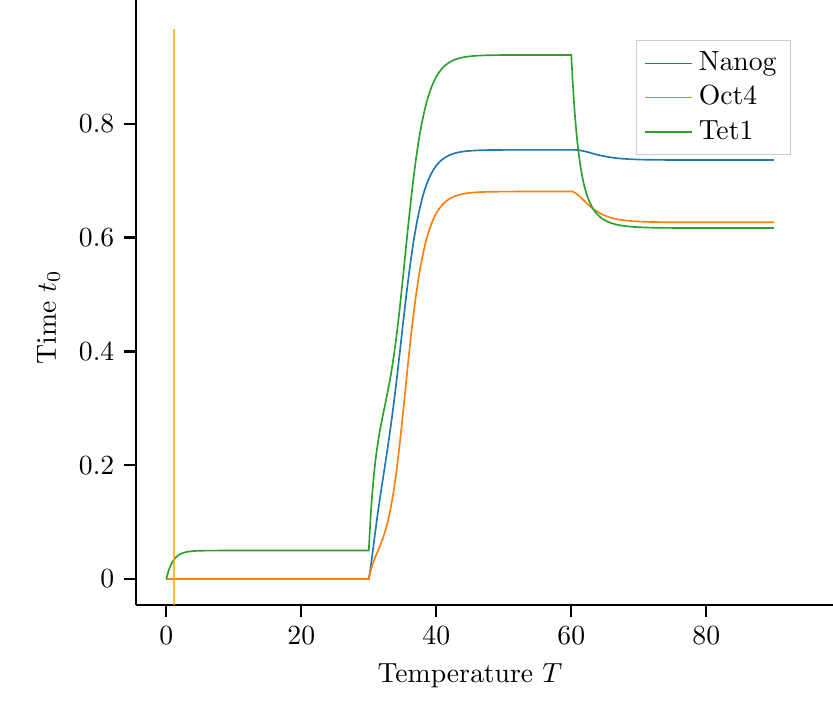
\begin{tikzpicture}

\definecolor{darkgray176}{RGB}{176,176,176}
\definecolor{darkorange25512714}{RGB}{255,127,14}
\definecolor{forestgreen4416044}{RGB}{44,160,44}
\definecolor{lightgray204}{RGB}{204,204,204}
\definecolor{orange}{RGB}{255,165,0}
\definecolor{steelblue31119180}{RGB}{31,119,180}

\begin{axis}[
legend cell align={left},
legend style={fill opacity=0.8, draw opacity=1, text opacity=1, draw=lightgray204},
tick align=outside,
tick pos=left,
x grid style={darkgray176},
xlabel={Temperature \(\displaystyle T\)},
xmin=-4.5, xmax=94.5,
xtick style={color=black},
y grid style={darkgray176},
ylabel={Time \(\displaystyle t_0\)},
ymin=-0.0460446703808976, ymax=0.966938077998851,
ytick style={color=black}
]
\addplot [semithick, steelblue31119180]
table {%
0 0
0.0001 0
0.0011 0
0.0111 0
0.1111 0
0.2111 0
0.3111 0
0.4111 0
0.5111 0
0.6111 0
0.7111 0
0.8111 0
0.9111 0
1.0111 0
1.1111 0
1.2111 0
1.3111 0
1.4111 0
1.5111 0
1.6111 0
1.7111 0
1.8111 0
1.9111 0
2.0111 0
2.1111 0
2.2111 0
2.3111 0
2.4111 0
2.5111 0
2.6111 0
2.7111 0
2.8111 0
2.9111 0
3.0111 0
3.1111 0
3.2111 0
3.3111 0
3.4111 0
3.5111 0
3.6111 0
3.7111 0
3.8111 0
3.9111 0
4.0111 0
4.1111 0
4.2111 0
4.3111 0
4.4111 0
4.5111 0
4.6111 0
4.7111 0
4.8111 0
4.9111 0
5.0111 0
5.1111 0
5.2111 0
5.3111 0
5.4111 0
5.5111 0
5.6111 0
5.7111 0
5.8111 0
5.9111 0
6.0111 0
6.1111 0
6.21109999999999 0
6.31109999999999 0
6.41109999999999 0
6.51109999999999 0
6.61109999999999 0
6.71109999999999 0
6.81109999999999 0
6.91109999999999 0
7.01109999999999 0
7.11109999999999 0
7.21109999999999 0
7.31109999999999 0
7.41109999999999 0
7.51109999999999 0
7.61109999999999 0
7.71109999999999 0
7.81109999999999 0
7.91109999999999 0
8.01109999999999 0
8.11109999999999 0
8.21109999999999 0
8.31109999999999 0
8.41109999999999 0
8.51109999999999 0
8.61109999999999 0
8.71109999999999 0
8.81109999999999 0
8.91109999999999 0
9.01109999999998 0
9.11109999999998 0
9.21109999999998 0
9.31109999999998 0
9.41109999999998 0
9.51109999999998 0
9.61109999999998 0
9.71109999999998 0
9.81109999999998 0
9.91109999999998 0
10.0111 0
10.1111 0
10.2111 0
10.3111 0
10.4111 0
10.5111 0
10.6111 0
10.7111 0
10.8111 0
10.9111 0
11.0111 0
11.1111 0
11.2111 0
11.3111 0
11.4111 0
11.5111 0
11.6111 0
11.7111 0
11.8111 0
11.9111 0
12.0111 0
12.1111 0
12.2111 0
12.3111 0
12.4111 0
12.5111 0
12.6111 0
12.7111 0
12.8111 0
12.9111 0
13.0111 0
13.1111 0
13.2111 0
13.3111 0
13.4111 0
13.5111 0
13.6111 0
13.7111 0
13.8111 0
13.9111 0
14.0111 0
14.1111 0
14.2111 0
14.3111 0
14.4111 0
14.5111 0
14.6111 0
14.7111 0
14.8111 0
14.9111 0
15.0111 0
15.1111 0
15.2111 0
15.3111 0
15.4111 0
15.5111 0
15.6111 0
15.7111 0
15.8111 0
15.9111 0
16.0111 0
16.1111 0
16.2111 0
16.3111 0
16.4111 0
16.5111 0
16.6111 0
16.7111 0
16.8111 0
16.9111 0
17.0111 0
17.1111 0
17.2111 0
17.3111 0
17.4111 0
17.5111 0
17.6111 0
17.7111 0
17.8111 0
17.9111 0
18.0111 0
18.1111 0
18.2111 0
18.3111 0
18.4111 0
18.5111 0
18.6111 0
18.7111 0
18.8111 0
18.9111 0
19.0111 0
19.1111 0
19.2111 0
19.3111 0
19.4111 0
19.5111 0
19.6111 0
19.7111 0
19.8111 0
19.9111 0
20.0111 0
20.1111 0
20.2111 0
20.3111 0
20.4111 0
20.5111 0
20.6111 0
20.7111 0
20.8111 0
20.9111 0
21.0111 0
21.1111 0
21.2111 0
21.3111 0
21.4111 0
21.5111 0
21.6111 0
21.7111 0
21.8111 0
21.9111 0
22.0111 0
22.1111 0
22.2111 0
22.3111 0
22.4111000000001 0
22.5111000000001 0
22.6111000000001 0
22.7111000000001 0
22.8111000000001 0
22.9111000000001 0
23.0111000000001 0
23.1111000000001 0
23.2111000000001 0
23.3111000000001 0
23.4111000000001 0
23.5111000000001 0
23.6111000000001 0
23.7111000000001 0
23.8111000000001 0
23.9111000000001 0
24.0111000000001 0
24.1111000000001 0
24.2111000000001 0
24.3111000000001 0
24.4111000000001 0
24.5111000000001 0
24.6111000000001 0
24.7111000000001 0
24.8111000000001 0
24.9111000000001 0
25.0111000000001 0
25.1111000000001 0
25.2111000000001 0
25.3111000000001 0
25.4111000000001 0
25.5111000000001 0
25.6111000000001 0
25.7111000000001 0
25.8111000000001 0
25.9111000000001 0
26.0111000000001 0
26.1111000000001 0
26.2111000000001 0
26.3111000000001 0
26.4111000000001 0
26.5111000000001 0
26.6111000000001 0
26.7111000000001 0
26.8111000000001 0
26.9111000000001 0
27.0111000000001 0
27.1111000000001 0
27.2111000000001 0
27.3111000000001 0
27.4111000000001 0
27.5111000000001 0
27.6111000000001 0
27.7111000000001 0
27.8111000000001 0
27.9111000000001 0
28.0111000000001 0
28.1111000000001 0
28.2111000000001 0
28.3111000000001 0
28.4111000000001 0
28.5111000000001 0
28.6111000000001 0
28.7111000000001 0
28.8111000000001 0
28.9111000000001 0
29.0111000000001 0
29.1111000000001 0
29.2111000000001 0
29.3111000000001 0
29.4111000000002 0
29.5111000000002 0
29.6111000000002 0
29.7111000000002 0
29.8111000000002 0
29.9111000000002 0
30 0
30 0
30.0115348003323 0.00070129486902565
30.1115348003323 0.0074713537807524
30.2115348003323 0.0152313305944161
30.3115348003323 0.0236846089484518
30.4115348003323 0.0325951158909974
30.5115348003323 0.0417774747941581
30.6115348003323 0.051088832552304
30.7115348003323 0.0604218236441233
30.8115348003323 0.0696984059774012
30.9115348003323 0.0788644534789487
31.0115348003323 0.0878850562156866
31.1115348003323 0.0967404956141111
31.2115348003323 0.105422856142046
31.3115348003323 0.11393322198154
31.4115348003323 0.122279396249071
31.5115348003323 0.130474074398911
31.6115348003323 0.138533402766155
31.7115348003323 0.146475856616248
31.8115348003323 0.154321378080348
31.9115348003323 0.162090721645049
32.0115348003323 0.169804962445913
32.1115348003323 0.177485129850553
32.2115348003323 0.185151935357833
32.3115348003323 0.192825569539665
32.4115348003323 0.200525547599228
32.5115348003323 0.208270587181701
32.6115348003323 0.21607850545859
32.7115348003323 0.223966125338303
32.8115348003323 0.231949183057705
32.9115348003323 0.240042231496859
33.0115348003323 0.248258535432185
33.1115348003323 0.256609956682551
33.2115348003323 0.265106828766706
33.3115348003323 0.273757822311134
33.4115348003323 0.282569804027973
33.5115348003323 0.291547693595709
33.6115348003324 0.300694324162289
33.7115348003324 0.310010313365565
33.8115348003324 0.319493952623955
33.9115348003324 0.329141122878089
34.0115348003324 0.338945244858511
34.1115348003324 0.348897271240655
34.2115348003324 0.358985726699871
34.3115348003324 0.369196799933093
34.4115348003324 0.379514489277374
34.5115348003324 0.389920800803011
34.6115348003324 0.400395994915479
34.7115348003324 0.410918874815231
34.8115348003324 0.421467107879009
34.9115348003324 0.432017569341321
35.0115348003324 0.442546696703517
35.1115348003324 0.453030843131279
35.2115348003324 0.46344661868592
35.3115348003324 0.473771209463896
35.4115348003324 0.483982666433385
35.5115348003324 0.494060157770806
35.6115348003324 0.503984180626481
35.7115348003324 0.513736730319687
35.8115348003324 0.523301426845729
35.9115348003324 0.532663600178914
36.0115348003324 0.541810337124623
36.1115348003324 0.550730493396908
36.2115348003324 0.559414675190261
36.3115348003324 0.567855194811183
36.4115348003324 0.576046004984307
36.5115348003324 0.583982616301743
36.6115348003324 0.591662001994655
36.7115348003324 0.59908249382016
36.8115348003324 0.60624367241501
36.9115348003324 0.613146255003283
37.0115348003324 0.619791982883704
37.1115348003324 0.626183510681831
37.2115348003324 0.63232429894536
37.3115348003324 0.638218511294653
37.4115348003324 0.643870917018793
37.5115348003324 0.649286799730402
37.6115348003324 0.65447187245875
37.7115348003324 0.659432199367356
37.8115348003324 0.664174124125583
37.9115348003324 0.66870420483969
38.0115348003324 0.673029155353012
38.1115348003324 0.677155792653535
38.2115348003324 0.68109099007612
38.3115348003324 0.684841635952613
38.4115348003324 0.688414597342924
38.5115348003324 0.6918166884711
38.6115348003324 0.695054643490224
38.7115348003324 0.698135093206435
38.8115348003324 0.701064545404059
38.9115348003324 0.703849368429139
39.0115348003324 0.706495777706579
39.1115348003324 0.709009824885648
39.2115348003324 0.711397389329028
39.3115348003324 0.71366417168139
39.4115348003324 0.715815689274068
39.5115348003324 0.717857273142608
39.6115348003324 0.71979406645342
39.7115348003324 0.721631024154298
39.8115348003324 0.723372913681145
39.9115348003324 0.725024316569702
40.0115348003324 0.726589630836425
40.1115348003324 0.728073074006877
40.2115348003324 0.729478686683147
40.3115348003324 0.730810336553823
40.4115348003324 0.732071722761081
40.5115348003324 0.733266380549478
40.6115348003324 0.734397686130136
40.7115348003325 0.735468861702265
40.8115348003325 0.736482980581378
40.9115348003325 0.737442972390271
41.0115348003325 0.738351628274814
41.1115348003325 0.739211606111978
41.2115348003325 0.740025435682317
41.3115348003325 0.740795523783369
41.4115348003325 0.741524159264239
41.5115348003325 0.742213517964966
41.6115348003325 0.742865667547233
41.7115348003325 0.743482572205577
41.8115348003325 0.744066097250548
41.9115348003325 0.744618013557235
42.0115348003325 0.745140001874358
42.1115348003325 0.745633656990583
42.2115348003325 0.746100491756068
42.3115348003325 0.746541940958335
42.4115348003325 0.746959365052542
42.5115348003325 0.747354053747042
42.6115348003325 0.747727229445793
42.7115348003325 0.748080050549781
42.8115348003325 0.748413614620071
42.9115348003325 0.748728961405517
43.0115348003325 0.749027075738447
43.1115348003325 0.749308890301923
43.2115348003325 0.749575288272327
43.3115348003325 0.749827105841201
43.4115348003325 0.75006513462033
43.5115348003325 0.750290123934146
43.6115348003325 0.750502783003536
43.7115348003325 0.750703783025139
43.8115348003325 0.750893759150215
43.9115348003325 0.751073312367074
44.0115348003325 0.751243011291065
44.1115348003325 0.751403393865965
44.2115348003325 0.751554968980611
44.3115348003325 0.751698218004445
44.4115348003325 0.751833596245606
44.5115348003325 0.751961534335034
44.6115348003325 0.752082439540014
44.7115348003325 0.752196697010396
44.8115348003325 0.752304670960673
44.9115348003325 0.752406705790961
45.0115348003325 0.752503127149799
45.1115348003325 0.752594242941599
45.2115348003325 0.752680344281428
45.3115348003325 0.75276170639974
45.4115348003325 0.752838589499514
45.5115348003325 0.752911239568182
45.6115348003325 0.752979889146622
45.7115348003325 0.753044758057384
45.8115348003325 0.753106054094205
45.9115348003325 0.753163973674817
46.0115348003325 0.753218702458899
46.1115348003325 0.753270415932996
46.2115348003325 0.753319279964104
46.3115348003325 0.753365451323536
46.4115348003325 0.753409078182647
46.5115348003325 0.753450300581861
46.6115348003325 0.753489250874421
46.7115348003325 0.753526054146179
46.8115348003325 0.753560828612703
46.9115348003325 0.75359368599489
47.0115348003325 0.753624731874236
47.1115348003325 0.753654066028833
47.2115348003325 0.753681782751132
47.3115348003325 0.753707971148439
47.4115348003325 0.753732715427062
47.5115348003325 0.753756095161006
47.6115348003325 0.753778185546015
47.7115348003326 0.753799057639781
47.8115348003326 0.753818778589038
47.9115348003326 0.753837411844269
48.0115348003326 0.753855017362678
48.1115348003326 0.753871651800074
48.2115348003326 0.753887368692262
48.3115348003326 0.753902218626509
48.4115348003326 0.753916249403625
48.5115348003326 0.753929506191168
48.6115348003326 0.753942031668257
48.7115348003326 0.753953866162445
48.8115348003326 0.753965047779091
48.9115348003326 0.753975612523635
49.0115348003326 0.753985594417158
49.1115348003326 0.753995025605612
49.2115348003326 0.754003936463041
49.3115348003326 0.754012355689139
49.4115348003326 0.754020310401449
49.5115348003326 0.75402782622249
49.6115348003326 0.754034927362107
49.7115348003326 0.75404163669528
49.8115348003326 0.754047975835666
49.9115348003326 0.75405396520509
50.0115348003326 0.754059624099214
50.1115348003326 0.754064970749597
50.2115348003326 0.754070022382337
50.3115348003326 0.754074795273483
50.4115348003326 0.754079304801405
50.5115348003326 0.754083565496269
50.6115348003326 0.754087591086801
50.7115348003326 0.754091394544467
50.8115348003326 0.754094988125221
50.9115348003326 0.754098383408957
51.0115348003326 0.754101591336785
51.1115348003326 0.754104622246252
51.2115348003326 0.754107485904628
51.3115348003326 0.754110191540354
51.4115348003326 0.754112747872752
51.5115348003326 0.754115163140111
51.6115348003326 0.754117445126211
51.7115348003326 0.754119601185394
51.8115348003326 0.754121638266249
51.9115348003326 0.754123562933992
52.0115348003326 0.754125381391613
52.1115348003326 0.754127099499859
52.2115348003326 0.75412872279611
52.3115348003326 0.754130256512215
52.4115348003326 0.754131705591354
52.5115348003326 0.754133074703955
52.6115348003326 0.754134368262746
52.7115348003326 0.754135590436969
52.8115348003326 0.754136745165815
52.9115348003326 0.754137836171114
53.0115348003326 0.75413886696933
53.1115348003326 0.754139840882889
53.2115348003326 0.754140761050884
53.3115348003326 0.754141630439192
53.4115348003326 0.754142451850033
53.5115348003326 0.754143227930994
53.6115348003326 0.754143961183566
53.7115348003326 0.754144653971203
53.8115348003326 0.75414530852694
53.9115348003326 0.754145926960587
54.0115348003326 0.75414651126553
54.1115348003326 0.754147063325153
54.2115348003326 0.754147584918912
54.3115348003326 0.754148077728064
54.4115348003326 0.754148543341091
54.5115348003326 0.754148983258816
54.6115348003326 0.754149398899241
54.7115348003327 0.754149791602116
54.8115348003327 0.75415016263326
54.9115348003327 0.754150513188638
55.0115348003327 0.754150844398217
55.1115348003327 0.754151157329606
55.2115348003327 0.7541514529915
55.3115348003327 0.754151732336928
55.4115348003327 0.754151996266328
55.5115348003327 0.754152245630446
55.6115348003327 0.75415248123308
55.7115348003327 0.75415270383367
55.8115348003327 0.754152914149747
55.9115348003327 0.754153112859244
56.0115348003327 0.754153300602683
56.1115348003327 0.754153477985236
56.2115348003327 0.754153645578683
56.3115348003327 0.754153803923244
56.4115348003327 0.754153953529333
56.5115348003327 0.75415409487919
56.6115348003327 0.754154228428447
56.7115348003327 0.754154354607591
56.8115348003327 0.754154473823349
56.9115348003327 0.754154586460005
57.0115348003327 0.754154692880637
57.1115348003327 0.754154793428283
57.2115348003327 0.754154888427053
57.3115348003327 0.754154978183169
57.4115348003327 0.754155062985955
57.5115348003327 0.754155143108766
57.6115348003327 0.754155218809874
57.7115348003327 0.754155290333297
57.8115348003327 0.754155357909586
57.9115348003327 0.754155421756571
58.0115348003327 0.754155482080058
58.1115348003327 0.754155539074497
58.2115348003327 0.754155592923606
58.3115348003327 0.754155643800966
58.4115348003327 0.754155691870576
58.5115348003327 0.754155737287387
58.6115348003327 0.754155780197797
58.7115348003327 0.754155820740127
58.8115348003327 0.754155859045062
58.9115348003327 0.754155895236077
59.0115348003327 0.754155929429831
59.1115348003327 0.754155961736547
59.2115348003327 0.754155992260363
59.3115348003327 0.754156021099673
59.4115348003327 0.754156048347438
59.5115348003327 0.754156074091489
59.6115348003327 0.754156098414813
59.7115348003327 0.754156121395814
59.8115348003327 0.75415614310857
59.9115348003327 0.754156163623072
60 0.754156180825457
60 0.754156180825457
60.1 0.754155411274351
60.2 0.754150184715445
60.3 0.754136755804323
60.4 0.754112082360919
60.5 0.754073751629896
60.6 0.754019911922564
60.7 0.753949209142016
60.8 0.753860727836864
60.9 0.753753936529841
61 0.75362863713339
61.1 0.753484918302961
61.2 0.753323112597191
61.3 0.75314375731869
61.4 0.752947558904838
61.5 0.752735360728681
61.6 0.75250811415869
61.7 0.752266852714878
61.8 0.752012669148755
61.9 0.751746695266916
62 0.751470084312823
62.1 0.751183995718825
62.2 0.750889582040575
62.3 0.750587977888355
62.4 0.75028029067435
62.5 0.749967593001063
62.6 0.749650916523647
62.7 0.749331247127541
62.8 0.749009521272168
62.9 0.748686623361303
63 0.748363384010805
63.1 0.74804057909457
63.2 0.747718929459567
63.3 0.74739910121062
63.4 0.747081706475007
63.5 0.746767304565956
63.6000000000001 0.746456403472617
63.7000000000001 0.746149461612084
63.8000000000001 0.74584688978647
63.9000000000001 0.745549053294925
64.0000000000001 0.745256274156835
64.1000000000001 0.744968833408212
64.2 0.744686973438566
64.3 0.744410900340337
64.4 0.744140786247219
64.5 0.743876771641603
64.6 0.743618967614752
64.7 0.743367458066407
64.8 0.743122301833154
64.9 0.742883534737298
65 0.742651171550002
65.1 0.742425207864235
65.2 0.742205621874658
65.3 0.741992376062814
65.4 0.741785418787194
65.5 0.741584685778614
65.6 0.741390101542173
65.7 0.741201580667684
65.8 0.741019029050994
65.8999999999999 0.740842345029026
65.9999999999999 0.740671420431686
66.0999999999999 0.740506141554043
66.1999999999999 0.740346390052318
66.2999999999999 0.740192043767373
66.3999999999999 0.740042977479399
66.4999999999999 0.73989906359757
66.5999999999999 0.739760172788358
66.6999999999999 0.739626174546186
66.7999999999999 0.739496937710014
66.8999999999999 0.739372330929327
66.9999999999999 0.739252223082947
67.0999999999999 0.739136483653884
67.1999999999999 0.739024983063393
67.2999999999999 0.738917592967193
67.3999999999999 0.738814186516714
67.4999999999999 0.738714638588075
67.5999999999999 0.738618825981331
67.6999999999998 0.738526627592435
67.7999999999998 0.738437924560156
67.8999999999998 0.738352600390117
67.9999999999998 0.738270541057932
68.0999999999998 0.738191635093339
68.1999999999998 0.738115773647043
68.2999999999998 0.738042850541925
68.3999999999998 0.737972762310121
68.4999999999998 0.73790540821736
68.5999999999998 0.737840690275883
68.6999999999998 0.737778513247127
68.7999999999998 0.73771878463529
68.8999999999998 0.737661414672801
68.9999999999998 0.737606316298623
69.0999999999998 0.737553405130267
69.1999999999998 0.737502599430293
69.2999999999998 0.73745382006803
69.3999999999997 0.737406990477169
69.4999999999997 0.737362036609836
69.5999999999997 0.737318886887686
69.6999999999997 0.737277472150519
69.7999999999997 0.737237725602868
69.8999999999997 0.737199582758961
69.9999999999997 0.737162981386427
70.0999999999997 0.737127861449078
70.1999999999997 0.737094165049054
70.2999999999997 0.737061836368611
70.3999999999997 0.737030821611765
70.4999999999997 0.737001068946024
70.5999999999997 0.736972528444381
70.6999999999997 0.736945152027734
70.7999999999997 0.736918893407875
70.8999999999997 0.736893708031171
70.9999999999997 0.736869553023058
71.0999999999997 0.736846387133418
71.1999999999996 0.736824170682938
71.2999999999996 0.736802865510512
71.3999999999996 0.736782434921732
71.4999999999996 0.73676284363853
71.5999999999996 0.736744057749992
71.6999999999996 0.73672604466438
71.7999999999996 0.736708773062379
71.8999999999996 0.736692212851587
71.9999999999996 0.736676335122249
72.0999999999996 0.736661112104244
72.1999999999996 0.736646517125324
72.2999999999996 0.736632524570591
72.3999999999996 0.736619109843208
72.4999999999996 0.736606249326337
72.5999999999996 0.736593920346278
72.6999999999996 0.736582101136793
72.7999999999996 0.736570770804609
72.8999999999996 0.736559909296057
72.9999999999995 0.736549497364843
73.0999999999995 0.736539516540916
73.1999999999995 0.736529949100415
73.2999999999995 0.73652077803666
73.3999999999995 0.736511987032177
73.4999999999995 0.736503560431709
73.5999999999995 0.736495483216208
73.6999999999995 0.736487740977763
73.7999999999995 0.736480319895448
73.8999999999995 0.736473206712061
73.9999999999995 0.73646638871172
74.0999999999995 0.736459853698304
74.1999999999995 0.736453589974696
74.2999999999995 0.736447586322815
74.3999999999995 0.736441831984403
74.4999999999995 0.736436316642551
74.5999999999995 0.736431030403925
74.6999999999994 0.736425963781685
74.7999999999994 0.736421107679062
74.8999999999994 0.736416453373571
74.9999999999994 0.736411992501844
75.0999999999994 0.736407717045053
75.1999999999994 0.736403619314909
75.2999999999994 0.736399691940206
75.3999999999994 0.736395927853906
75.4999999999994 0.736392320280728
75.5999999999994 0.736388862725236
75.6999999999994 0.736385548960396
75.7999999999994 0.736382373016592
75.8999999999994 0.736379329171088
75.9999999999994 0.736376411937899
76.0999999999994 0.736373616058083
76.1999999999994 0.736370936490416
76.2999999999994 0.736368368402444
76.3999999999994 0.7363659071619
76.4999999999993 0.736363548328463
76.5999999999993 0.736361287645858
76.6999999999993 0.736359121034269
76.7999999999993 0.736357044583066
76.8999999999993 0.736355054543827
76.9999999999993 0.736353147323643
77.0999999999993 0.736351319478695
77.1999999999993 0.736349567708099
77.2999999999993 0.736347888847996
77.3999999999993 0.736346279865887
77.4999999999993 0.7363447378552
77.5999999999993 0.736343260030083
77.6999999999993 0.7363418437204
77.7999999999993 0.736340486366947
77.8999999999993 0.736339185516855
77.9999999999993 0.736337938819181
78.0999999999993 0.73633674402069
78.1999999999992 0.736335598961801
78.2999999999992 0.736334501572705
78.3999999999992 0.736333449869641
78.4999999999992 0.736332441951328
78.5999999999992 0.736331475995541
78.6999999999992 0.736330550255832
78.7999999999992 0.736329663058382
78.8999999999992 0.736328812798989
78.9999999999992 0.736327997940176
79.0999999999992 0.736327217008418
79.1999999999992 0.736326468591491
79.2999999999992 0.736325751335917
79.3999999999992 0.736325063944533
79.4999999999992 0.736324405174144
79.5999999999992 0.736323773833283
79.6999999999992 0.736323168780058
79.7999999999992 0.736322588920098
79.8999999999992 0.73632203320457
79.9999999999991 0.736321500628291
80.0999999999991 0.736320990227909
80.1999999999991 0.736320501080168
80.2999999999991 0.736320032300236
80.3999999999991 0.73631958304011
80.4999999999991 0.736319152487084
80.5999999999991 0.736318739862279
80.6999999999991 0.736318344419237
80.7999999999991 0.736317965442573
80.8999999999991 0.73631760224668
80.9999999999991 0.736317254174494
81.0999999999991 0.736316920596301
81.1999999999991 0.736316600908604
81.2999999999991 0.736316294533028
81.3999999999991 0.73631600091528
81.4999999999991 0.736315719524139
81.5999999999991 0.736315449850503
81.6999999999991 0.736315191406465
81.799999999999 0.736314943724431
81.899999999999 0.736314706356276
81.999999999999 0.73631447887253
82.099999999999 0.736314260861609
82.199999999999 0.73631405192906
82.299999999999 0.736313851696858
82.399999999999 0.736313659802716
82.499999999999 0.736313475899432
82.599999999999 0.736313299654258
82.699999999999 0.736313130748306
82.799999999999 0.736312968875962
82.899999999999 0.736312813744338
82.999999999999 0.736312665072742
83.099999999999 0.73631252259217
83.199999999999 0.736312386044818
83.299999999999 0.736312255183617
83.399999999999 0.736312129771788
83.4999999999989 0.736312009582409
83.5999999999989 0.736311894398007
83.6999999999989 0.736311784010166
83.7999999999989 0.736311678219149
83.8999999999989 0.736311576833534
83.9999999999989 0.736311479669871
84.0999999999989 0.736311386552349
84.1999999999989 0.736311297312479
84.2999999999989 0.736311211788786
84.3999999999989 0.736311129826521
84.4999999999989 0.736311051277378
84.5999999999989 0.736310975999226
84.6999999999989 0.736310903855854
84.7999999999989 0.736310834716722
84.8999999999989 0.736310768456726
84.9999999999989 0.736310704955972
85.0999999999989 0.736310644099558
85.1999999999989 0.736310585777368
85.2999999999988 0.736310529883871
85.3999999999988 0.736310476317928
85.4999999999988 0.736310424982615
85.5999999999988 0.736310375785043
85.6999999999988 0.736310328636191
85.7999999999988 0.736310283450745
85.8999999999988 0.736310240146943
85.9999999999988 0.736310198646429
86.0999999999988 0.736310158874109
86.1999999999988 0.736310120758017
86.2999999999988 0.736310084229182
86.3999999999988 0.736310049221508
86.4999999999988 0.736310015671649
86.5999999999988 0.736309983518898
86.6999999999988 0.736309952705075
86.7999999999988 0.736309923174424
86.8999999999988 0.73630989487351
86.9999999999987 0.736309867751124
87.0999999999987 0.736309841758188
87.1999999999987 0.736309816847669
87.2999999999987 0.736309792974493
87.3999999999987 0.736309770095461
87.4999999999987 0.736309748169174
87.5999999999987 0.736309727155959
87.6999999999987 0.736309707017791
87.7999999999987 0.736309687718231
87.8999999999987 0.736309669222359
87.9999999999987 0.736309651496705
88.0999999999987 0.736309634509196
88.1999999999987 0.736309618229094
88.2999999999987 0.73630960262694
88.3999999999987 0.736309587674502
88.4999999999987 0.736309573344725
88.5999999999987 0.736309559611679
88.6999999999987 0.736309546450514
88.7999999999986 0.736309533837417
88.8999999999986 0.736309521749564
88.9999999999986 0.736309510165082
89.0999999999986 0.736309499063009
89.1999999999986 0.736309488423258
89.2999999999986 0.736309478226574
89.3999999999986 0.736309468454509
89.4999999999986 0.736309459089379
89.5999999999986 0.736309450114239
89.6999999999986 0.736309441512848
89.7999999999986 0.736309433269643
89.8999999999986 0.736309425369708
89.9999999999986 0.736309417798747
90 0.736309417798747
};
\addlegendentry{Nanog}
\addplot [semithick, darkorange25512714]
table {%
0 0
0.0001 0
0.0011 0
0.0111 0
0.1111 0
0.2111 0
0.3111 0
0.4111 0
0.5111 0
0.6111 0
0.7111 0
0.8111 0
0.9111 0
1.0111 0
1.1111 0
1.2111 0
1.3111 0
1.4111 0
1.5111 0
1.6111 0
1.7111 0
1.8111 0
1.9111 0
2.0111 0
2.1111 0
2.2111 0
2.3111 0
2.4111 0
2.5111 0
2.6111 0
2.7111 0
2.8111 0
2.9111 0
3.0111 0
3.1111 0
3.2111 0
3.3111 0
3.4111 0
3.5111 0
3.6111 0
3.7111 0
3.8111 0
3.9111 0
4.0111 0
4.1111 0
4.2111 0
4.3111 0
4.4111 0
4.5111 0
4.6111 0
4.7111 0
4.8111 0
4.9111 0
5.0111 0
5.1111 0
5.2111 0
5.3111 0
5.4111 0
5.5111 0
5.6111 0
5.7111 0
5.8111 0
5.9111 0
6.0111 0
6.1111 0
6.21109999999999 0
6.31109999999999 0
6.41109999999999 0
6.51109999999999 0
6.61109999999999 0
6.71109999999999 0
6.81109999999999 0
6.91109999999999 0
7.01109999999999 0
7.11109999999999 0
7.21109999999999 0
7.31109999999999 0
7.41109999999999 0
7.51109999999999 0
7.61109999999999 0
7.71109999999999 0
7.81109999999999 0
7.91109999999999 0
8.01109999999999 0
8.11109999999999 0
8.21109999999999 0
8.31109999999999 0
8.41109999999999 0
8.51109999999999 0
8.61109999999999 0
8.71109999999999 0
8.81109999999999 0
8.91109999999999 0
9.01109999999998 0
9.11109999999998 0
9.21109999999998 0
9.31109999999998 0
9.41109999999998 0
9.51109999999998 0
9.61109999999998 0
9.71109999999998 0
9.81109999999998 0
9.91109999999998 0
10.0111 0
10.1111 0
10.2111 0
10.3111 0
10.4111 0
10.5111 0
10.6111 0
10.7111 0
10.8111 0
10.9111 0
11.0111 0
11.1111 0
11.2111 0
11.3111 0
11.4111 0
11.5111 0
11.6111 0
11.7111 0
11.8111 0
11.9111 0
12.0111 0
12.1111 0
12.2111 0
12.3111 0
12.4111 0
12.5111 0
12.6111 0
12.7111 0
12.8111 0
12.9111 0
13.0111 0
13.1111 0
13.2111 0
13.3111 0
13.4111 0
13.5111 0
13.6111 0
13.7111 0
13.8111 0
13.9111 0
14.0111 0
14.1111 0
14.2111 0
14.3111 0
14.4111 0
14.5111 0
14.6111 0
14.7111 0
14.8111 0
14.9111 0
15.0111 0
15.1111 0
15.2111 0
15.3111 0
15.4111 0
15.5111 0
15.6111 0
15.7111 0
15.8111 0
15.9111 0
16.0111 0
16.1111 0
16.2111 0
16.3111 0
16.4111 0
16.5111 0
16.6111 0
16.7111 0
16.8111 0
16.9111 0
17.0111 0
17.1111 0
17.2111 0
17.3111 0
17.4111 0
17.5111 0
17.6111 0
17.7111 0
17.8111 0
17.9111 0
18.0111 0
18.1111 0
18.2111 0
18.3111 0
18.4111 0
18.5111 0
18.6111 0
18.7111 0
18.8111 0
18.9111 0
19.0111 0
19.1111 0
19.2111 0
19.3111 0
19.4111 0
19.5111 0
19.6111 0
19.7111 0
19.8111 0
19.9111 0
20.0111 0
20.1111 0
20.2111 0
20.3111 0
20.4111 0
20.5111 0
20.6111 0
20.7111 0
20.8111 0
20.9111 0
21.0111 0
21.1111 0
21.2111 0
21.3111 0
21.4111 0
21.5111 0
21.6111 0
21.7111 0
21.8111 0
21.9111 0
22.0111 0
22.1111 0
22.2111 0
22.3111 0
22.4111000000001 0
22.5111000000001 0
22.6111000000001 0
22.7111000000001 0
22.8111000000001 0
22.9111000000001 0
23.0111000000001 0
23.1111000000001 0
23.2111000000001 0
23.3111000000001 0
23.4111000000001 0
23.5111000000001 0
23.6111000000001 0
23.7111000000001 0
23.8111000000001 0
23.9111000000001 0
24.0111000000001 0
24.1111000000001 0
24.2111000000001 0
24.3111000000001 0
24.4111000000001 0
24.5111000000001 0
24.6111000000001 0
24.7111000000001 0
24.8111000000001 0
24.9111000000001 0
25.0111000000001 0
25.1111000000001 0
25.2111000000001 0
25.3111000000001 0
25.4111000000001 0
25.5111000000001 0
25.6111000000001 0
25.7111000000001 0
25.8111000000001 0
25.9111000000001 0
26.0111000000001 0
26.1111000000001 0
26.2111000000001 0
26.3111000000001 0
26.4111000000001 0
26.5111000000001 0
26.6111000000001 0
26.7111000000001 0
26.8111000000001 0
26.9111000000001 0
27.0111000000001 0
27.1111000000001 0
27.2111000000001 0
27.3111000000001 0
27.4111000000001 0
27.5111000000001 0
27.6111000000001 0
27.7111000000001 0
27.8111000000001 0
27.9111000000001 0
28.0111000000001 0
28.1111000000001 0
28.2111000000001 0
28.3111000000001 0
28.4111000000001 0
28.5111000000001 0
28.6111000000001 0
28.7111000000001 0
28.8111000000001 0
28.9111000000001 0
29.0111000000001 0
29.1111000000001 0
29.2111000000001 0
29.3111000000001 0
29.4111000000002 0
29.5111000000002 0
29.6111000000002 0
29.7111000000002 0
29.8111000000002 0
29.9111000000002 0
30 0
30 0
30.0115348003323 0.000688111783925976
30.1115348003323 0.00633251224677741
30.2115348003323 0.0114417071605194
30.3115348003323 0.0160728709093962
30.4115348003323 0.0202837149216242
30.5115348003323 0.0241324323582999
30.6115348003323 0.0276766005889729
30.7115348003323 0.0309717206486731
30.8115348003323 0.0340698830235261
30.9115348003323 0.037018819811588
31.0115348003323 0.0398614169041925
31.1115348003323 0.0426356418609034
31.2115348003323 0.045374787921174
31.3115348003323 0.048107923565434
31.4115348003323 0.0508604506531327
31.5115348003323 0.0536546974725109
31.6115348003323 0.0565104968753765
31.7115348003323 0.0594457196264403
31.8115348003323 0.0624767478439632
31.9115348003323 0.0656188832583765
32.0115348003323 0.0688866909385501
32.1115348003323 0.0722942822108262
32.2115348003323 0.0758555416621301
32.3115348003323 0.0795843030971238
32.4115348003323 0.0834944786251329
32.5115348003323 0.0876001440350016
32.6115348003323 0.0919155825066926
32.7115348003323 0.0964552876618139
32.8115348003323 0.101233926079785
32.9115348003323 0.106266258785746
33.0115348003323 0.111567020922209
33.1115348003323 0.117150758913873
33.2115348003323 0.123031624981058
33.3115348003323 0.129223129895072
33.4115348003323 0.135737856415979
33.5115348003323 0.142587137888186
33.6115348003324 0.149780708916142
33.7115348003324 0.157326337758973
33.8115348003324 0.165229452855332
33.9115348003324 0.173492778437916
34.0115348003324 0.182115996195147
34.1115348003324 0.191095451049023
34.2115348003324 0.200423919045184
34.3115348003324 0.210090453888411
34.4115348003324 0.220080325742
34.5115348003324 0.230375061656488
34.6115348003324 0.240952591698279
34.7115348003324 0.251787498963172
34.8115348003324 0.262851365732788
34.9115348003324 0.274113202632005
35.0115348003324 0.28553994327732
35.1115348003324 0.297096983939411
35.2115348003324 0.30874874636764
35.3115348003324 0.320459242137663
35.4115348003324 0.332192618511933
35.5115348003324 0.343913668545837
35.6115348003324 0.355588291658515
35.7115348003324 0.367183894733183
35.8115348003324 0.378669727667408
35.9115348003324 0.390017150876942
36.0115348003324 0.40119983536772
36.1115348003324 0.412193898514144
36.2115348003324 0.422977980577236
36.3115348003324 0.433533268282465
36.4115348003324 0.443843472514226
36.5115348003324 0.453894767456806
36.6115348003324 0.463675698415143
36.7115348003324 0.473177065176948
36.8115348003324 0.482391787217192
36.9115348003324 0.491314756370603
37.0115348003324 0.499942681868008
37.1115348003324 0.508273931894642
37.2115348003324 0.516308375116568
37.3115348003324 0.52404722495814
37.4115348003324 0.531492888812918
37.5115348003324 0.538648823839541
37.6115348003324 0.545519400534684
37.7115348003324 0.552109774885342
37.8115348003324 0.558425769578159
37.9115348003324 0.564473764478389
38.0115348003324 0.570260596378921
38.1115348003324 0.575793467853963
38.2115348003324 0.581079864925717
38.3115348003324 0.586127483159734
38.4115348003324 0.590944161739895
38.5115348003324 0.59553782503205
38.6115348003324 0.599916431121997
38.7115348003324 0.604087926804757
38.8115348003324 0.608060208504866
38.9115348003324 0.611841088618878
39.0115348003324 0.615438266789217
39.1115348003324 0.618859305641111
39.2115348003324 0.62211161053997
39.3115348003324 0.625202412954213
39.4115348003324 0.628138757037013
39.5115348003324 0.630927489069206
39.6115348003324 0.633575249433955
39.7115348003324 0.636088466821359
39.8115348003324 0.638473354387659
39.9115348003324 0.640735907618907
40.0115348003324 0.642881903672679
40.1115348003324 0.64491690199365
40.2115348003324 0.646846246019502
40.3115348003324 0.648675065812793
40.4115348003324 0.650408281471998
40.5115348003324 0.652050607191088
40.6115348003324 0.653606555851797
40.7115348003325 0.655080444046108
40.8115348003325 0.65647639743871
40.9115348003325 0.657798356390187
41.0115348003325 0.659050081771635
41.1115348003325 0.660235160910363
41.2115348003325 0.661357013614347
41.3115348003325 0.662418898230287
41.4115348003325 0.663423917696543
41.5115348003325 0.664375025557922
41.6115348003325 0.665275031914377
41.7115348003325 0.666126609280158
41.8115348003325 0.666932298333948
41.9115348003325 0.667694513544005
42.0115348003325 0.66841554865543
42.1115348003325 0.669097582029355
42.2115348003325 0.669742681826237
42.3115348003325 0.67035281102746
42.4115348003325 0.67092983229127
42.5115348003325 0.671475512640573
42.6115348003325 0.671991527981463
42.7115348003325 0.672479467452494
42.8115348003325 0.672940837605636
42.9115348003325 0.673377066420705
43.0115348003325 0.673789507155715
43.1115348003325 0.674179442036173
43.2115348003325 0.674548085786785
43.3115348003325 0.674896589009438
43.4115348003325 0.675226041411588
43.5115348003325 0.675537474889434
43.6115348003325 0.675831866470402
43.7115348003325 0.67611014111959
43.8115348003325 0.676373174414905
43.9115348003325 0.676621795095622
44.0115348003325 0.676856787489136
44.1115348003325 0.677078893820628
44.2115348003325 0.677288816410312
44.3115348003325 0.67748721976288
44.4115348003325 0.677674732553652
44.5115348003325 0.677851949515876
44.6115348003325 0.678019433233455
44.7115348003325 0.678177715843342
44.8115348003325 0.678327300651634
44.9115348003325 0.678468663667338
45.0115348003325 0.678602255057614
45.1115348003325 0.678728500528174
45.2115348003325 0.678847802632386
45.3115348003325 0.678960542012501
45.4115348003325 0.679067078576271
45.5115348003325 0.679167752612128
45.6115348003325 0.67926288584592
45.7115348003325 0.679352782442113
45.8115348003325 0.67943772995222
45.9115348003325 0.67951800021311
46.0115348003325 0.679593850197718
46.1115348003325 0.679665522820575
46.2115348003325 0.679733247700466
46.3115348003325 0.679797241882412
46.4115348003325 0.679857710521058
46.5115348003325 0.679914847527485
46.6115348003325 0.679968836181319
46.7115348003325 0.680019849709968
46.8115348003325 0.680068051836685
46.9115348003325 0.680113597299109
47.0115348003325 0.680156632339817
47.1115348003325 0.680197295170388
47.2115348003325 0.680235716410357
47.3115348003325 0.680272019502401
47.4115348003325 0.680306321105022
47.5115348003325 0.680338731463921
47.6115348003325 0.680369354763193
47.7115348003326 0.680398289457445
47.8115348003326 0.680425628585828
47.9115348003326 0.680451460068984
48.0115348003326 0.680475866989795
48.1115348003326 0.680498927858839
48.2115348003326 0.680520716865348
48.3115348003326 0.680541304114468
48.4115348003326 0.680560755851559
48.5115348003326 0.680579134674227
48.6115348003326 0.680596499732762
48.7115348003326 0.680612906919612
48.8115348003326 0.680628409048475
48.9115348003326 0.680643056023589
49.0115348003326 0.680656894999743
49.1115348003326 0.680669970533517
49.2115348003326 0.680682324726227
49.3115348003326 0.680693997359031
49.4115348003326 0.680705026020618
49.5115348003326 0.680715446227895
49.6115348003326 0.680725291540034
49.7115348003326 0.680734593666272
49.8115348003326 0.680743382567771
49.9115348003326 0.680751686553898
50.0115348003326 0.680759532373196
50.1115348003326 0.680766945299369
50.2115348003326 0.680773949212528
50.3115348003326 0.680780566675974
50.4115348003326 0.680786819008753
50.5115348003326 0.680792726354225
50.6115348003326 0.680798307744853
50.7115348003326 0.680803581163432
50.8115348003326 0.680808563600941
50.9115348003326 0.680813271111221
51.0115348003326 0.680817718862628
51.1115348003326 0.680821921186851
51.2115348003326 0.680825891625044
51.3115348003326 0.680829642971405
51.4115348003326 0.680833187314366
51.5115348003326 0.680836536075511
51.6115348003326 0.680839700046342
51.7115348003326 0.680842689423032
51.8115348003326 0.680845513839252
51.9115348003326 0.680848182397195
52.0115348003326 0.680850703696887
52.1115348003326 0.680853085863883
52.2115348003326 0.68085533657544
52.3115348003326 0.680857463085239
52.4115348003326 0.680859472246753
52.5115348003326 0.680861370535322
52.6115348003326 0.68086316406901
52.7115348003326 0.680864858628315
52.8115348003326 0.680866459674791
52.9115348003326 0.680867972368641
53.0115348003326 0.680869401585344
53.1115348003326 0.680870751931359
53.2115348003326 0.680872027758972
53.3115348003326 0.680873233180316
53.4115348003326 0.680874372080617
53.5115348003326 0.680875448130719
53.6115348003326 0.680876464798908
53.7115348003326 0.680877425362091
53.8115348003326 0.68087833291635
53.9115348003326 0.680879190386926
54.0115348003326 0.680880000537638
54.1115348003326 0.680880765979795
54.2115348003326 0.680881489180609
54.3115348003326 0.680882172471146
54.4115348003326 0.680882818053839
54.5115348003326 0.680883428009583
54.6115348003326 0.680884004304445
54.7115348003327 0.680884548795997
54.8115348003327 0.680885063239307
54.9115348003327 0.680885549292589
55.0115348003327 0.680886008522552
55.1115348003327 0.680886442409449
55.2115348003327 0.680886852351846
55.3115348003327 0.68088723967113
55.4115348003327 0.680887605615769
55.5115348003327 0.680887951365335
55.6115348003327 0.680888278034306
55.7115348003327 0.680888586675657
55.8115348003327 0.680888878284256
55.9115348003327 0.680889153800068
56.0115348003327 0.680889414111189
56.1115348003327 0.680889660056701
56.2115348003327 0.680889892429385
56.3115348003327 0.68089011197827
56.4115348003327 0.680890319411051
56.5115348003327 0.680890515396368
56.6115348003327 0.680890700565961
56.7115348003327 0.680890875516708
56.8115348003327 0.680891040812548
56.9115348003327 0.680891196986299
57.0115348003327 0.680891344541373
57.1115348003327 0.680891483953404
57.2115348003327 0.680891615671775
57.3115348003327 0.680891740121071
57.4115348003327 0.680891857702446
57.5115348003327 0.680891968794914
57.6115348003327 0.680892073756575
57.7115348003327 0.680892172925765
57.8115348003327 0.680892266622151
57.9115348003327 0.680892355147756
58.0115348003327 0.680892438787938
58.1115348003327 0.680892517812305
58.2115348003327 0.680892592475589
58.3115348003327 0.680892663018461
58.4115348003327 0.680892729668312
58.5115348003327 0.680892792639986
58.6115348003327 0.680892852136467
58.7115348003327 0.68089290834954
58.8115348003327 0.680892961460403
58.9115348003327 0.680893011640259
59.0115348003327 0.680893059050857
59.1115348003327 0.680893103845025
59.2115348003327 0.680893146167154
59.3115348003327 0.680893186153668
59.4115348003327 0.68089322393346
59.5115348003327 0.680893259628313
59.6115348003327 0.680893293353287
59.7115348003327 0.680893325217092
59.8115348003327 0.680893355322441
59.9115348003327 0.680893383766377
60 0.680893407617971
60 0.680893407617971
60.1 0.680816208030429
60.2 0.68059256301836
60.3 0.680234441823288
60.4 0.679753694119775
60.5 0.679161966085938
60.6 0.678470618882534
60.7 0.677690653412261
60.8 0.676832644075471
60.9 0.675906683187223
61 0.674922336827996
61.1 0.673888612187954
61.2 0.672813935930474
61.3 0.671706142728474
61.4 0.670572472893078
61.5 0.669419577891832
61.6 0.668253532517646
61.7 0.667079852496562
61.8 0.66590351639302
61.9 0.664728990769381
62 0.663560257669791
62.1 0.662400843617612
62.2 0.661253849433934
62.3 0.660121980297478
62.4 0.659007575570631
62.5 0.657912638010682
62.6 0.656838862068947
62.7 0.655787661053212
62.8 0.654760192991287
62.9 0.653757385086073
63 0.652779956696333
63.1 0.651828440813155
63.2 0.650903204030986
63.3 0.650004465034912
63.4 0.649132311643479
63.5 0.648286716459587
63.6000000000001 0.647467551191535
63.7000000000001 0.646674599712834
63.8000000000001 0.645907569933406
63.9000000000001 0.645166104556837
64.0000000000001 0.644449790798748
64.1000000000001 0.643758169140556
64.2 0.643090741191087
64.3 0.642446976726023
64.4 0.641826319972154
64.5 0.641228195200031
64.6 0.640652011685057
64.7 0.640097168093344
64.8 0.639563056344948
64.9 0.63904906500342
65 0.638554582236986
65.1 0.638078998393226
65.2 0.637621708225742
65.3 0.637182112808206
65.4 0.636759621168116
65.5 0.636353651669845
65.6 0.635963633173909
65.7 0.635589005996952
65.8 0.635229222694678
65.8999999999999 0.634883748687883
65.9999999999999 0.634552062749783
66.0999999999999 0.634233657371104
66.1999999999999 0.633928039017738
66.2999999999999 0.63363472829432
66.3999999999999 0.633353260025685
66.4999999999999 0.633083183266972
66.5999999999999 0.632824061251992
66.6999999999999 0.632575471288462
66.7999999999999 0.632337004607783
66.8999999999999 0.632108266176212
66.9999999999999 0.631888874473514
67.0999999999999 0.631678461244484
67.1999999999999 0.631476671228142
67.2999999999999 0.631283161868831
67.3999999999999 0.631097603012936
67.4999999999999 0.630919676594536
67.5999999999999 0.630749076312849
67.6999999999998 0.630585507304012
67.7999999999998 0.630428685809377
67.8999999999998 0.630278338842267
67.9999999999998 0.630134203854807
68.0999999999998 0.629996028406303
68.1999999999998 0.629863569834346
68.2999999999998 0.629736594929725
68.3999999999998 0.629614879615992
68.4999999999998 0.629498208634446
68.5999999999998 0.629386375235126
68.6999999999998 0.629279180874329
68.7999999999998 0.629176434919043
68.8999999999998 0.629077954358619
68.9999999999998 0.628983563523913
69.0999999999998 0.628893093814081
69.1999999999998 0.628806383431135
69.2999999999998 0.628723277122333
69.3999999999997 0.628643625930413
69.4999999999997 0.62856728695167
69.5999999999997 0.628494123101816
69.6999999999997 0.628424002889559
69.7999999999997 0.628356800197789
69.8999999999997 0.628292394072267
69.9999999999997 0.628230668517673
70.0999999999997 0.628171512300867
70.1999999999997 0.62811481876121
70.2999999999997 0.62806048562777
70.3999999999997 0.628008414843242
70.4999999999997 0.627958512394406
70.5999999999997 0.627910688148938
70.6999999999997 0.627864855698386
70.7999999999997 0.627820932207132
70.8999999999997 0.627778838267153
70.9999999999997 0.627738497758388
71.0999999999997 0.627699837714541
71.1999999999996 0.627662788194127
71.2999999999996 0.627627282156589
71.3999999999996 0.627593255343304
71.4999999999996 0.627560646163315
71.5999999999996 0.627529395583612
71.6999999999996 0.6274994470238
71.7999999999996 0.627470746254992
71.8999999999996 0.627443241302775
71.9999999999996 0.62741688235409
72.0999999999996 0.627391621667882
72.1999999999996 0.62736741348938
72.2999999999996 0.627344213967855
72.3999999999996 0.62732198107774
72.4999999999996 0.627300674542964
72.5999999999996 0.62728025576439
72.6999999999996 0.627260687750215
72.7999999999996 0.62724193504924
72.8999999999996 0.627223963686875
72.9999999999995 0.62720674110378
73.0999999999995 0.627190236097032
73.1999999999995 0.627174418763728
73.2999999999995 0.627159260446904
73.3999999999995 0.6271447336837
73.4999999999995 0.627130812155666
73.5999999999995 0.627117470641121
73.6999999999995 0.627104684969494
73.7999999999995 0.627092431977553
73.8999999999995 0.627080689467451
73.9999999999995 0.627069436166512
74.0999999999995 0.627058651688689
74.1999999999995 0.627048316497624
74.2999999999995 0.627038411871241
74.3999999999995 0.627028919867812
74.4999999999995 0.627019823293436
74.5999999999995 0.627011105670871
74.6999999999994 0.62700275120966
74.7999999999994 0.626994744777506
74.8999999999994 0.626987071872833
74.9999999999994 0.626979718598495
75.0999999999994 0.626972671636579
75.1999999999994 0.626965918224255
75.2999999999994 0.626959446130634
75.3999999999994 0.626953243634595
75.4999999999994 0.626947299503528
75.5999999999994 0.626941602972967
75.6999999999994 0.626936143727076
75.7999999999994 0.626930911879941
75.8999999999994 0.626925897957648
75.9999999999994 0.626921092881107
76.0999999999994 0.626916487949588
76.1999999999994 0.626912074824951
76.2999999999994 0.626907845516527
76.3999999999994 0.626903792366634
76.4999999999993 0.626899908036694
76.5999999999993 0.626896185493931
76.6999999999993 0.626892617998622
76.7999999999993 0.626889199091881
76.8999999999993 0.626885922583955
76.9999999999993 0.626882782543
77.0999999999993 0.626879773284335
77.1999999999993 0.626876889360138
77.2999999999993 0.626874125549571
77.3999999999993 0.626871476849324
77.4999999999993 0.626868938464544
77.5999999999993 0.626866505800148
77.6999999999993 0.626864174452499
77.7999999999993 0.626861940201423
77.8999999999993 0.626859799002567
77.9999999999993 0.626857746980069
78.0999999999993 0.626855780419537
78.1999999999992 0.626853895761321
78.2999999999992 0.626852089594062
78.3999999999992 0.626850358648515
78.4999999999992 0.626848699791626
78.5999999999992 0.626847110020855
78.6999999999992 0.626845586458742
78.7999999999992 0.626844126347691
78.8999999999992 0.626842727044977
78.9999999999992 0.626841386017959
79.0999999999992 0.626840100839496
79.1999999999992 0.626838869183547
79.2999999999992 0.626837688820963
79.3999999999992 0.626836557615446
79.4999999999992 0.626835473519684
79.5999999999992 0.626834434571641
79.6999999999992 0.626833438891007
79.7999999999992 0.62683248467579
79.8999999999992 0.626831570199055
79.9999999999991 0.626830693805799
80.0999999999991 0.626829853909949
80.1999999999991 0.626829048991497
80.2999999999991 0.626828277593742
80.3999999999991 0.626827538320657
80.4999999999991 0.62682682983436
80.5999999999991 0.626826150852689
80.6999999999991 0.626825500146888
80.7999999999991 0.626824876539375
80.8999999999991 0.626824278901614
80.9999999999991 0.626823706152072
81.0999999999991 0.626823157254259
81.1999999999991 0.626822631214855
81.2999999999991 0.626822127081909
81.3999999999991 0.626821643943117
81.4999999999991 0.626821180924171
81.5999999999991 0.626820737187175
81.6999999999991 0.62682031192913
81.799999999999 0.62681990438048
81.899999999999 0.626819513803717
81.999999999999 0.626819139492051
82.099999999999 0.626818780768124
82.199999999999 0.626818436982791
82.299999999999 0.62681810751394
82.399999999999 0.626817791765366
82.499999999999 0.626817489165698
82.599999999999 0.626817199167355
82.699999999999 0.626816921245566
82.799999999999 0.626816654897409
82.899999999999 0.626816399640912
82.999999999999 0.62681615501417
83.099999999999 0.626815920574518
83.199999999999 0.626815695897724
83.299999999999 0.626815480577224
83.399999999999 0.626815274223385
83.4999999999989 0.626815076462801
83.5999999999989 0.626814886937614
83.6999999999989 0.626814705304873
83.7999999999989 0.626814531235905
83.8999999999989 0.626814364415729
83.9999999999989 0.626814204542476
84.0999999999989 0.626814051326853
84.1999999999989 0.626813904491611
84.2999999999989 0.626813763771049
84.3999999999989 0.62681362891053
84.4999999999989 0.626813499666022
84.5999999999989 0.626813375803653
84.6999999999989 0.626813257099294
84.7999999999989 0.626813143338148
84.8999999999989 0.626813034314361
84.9999999999989 0.626812929830656
85.0999999999989 0.626812829697967
85.1999999999989 0.626812733735104
85.2999999999988 0.626812641768422
85.3999999999988 0.626812553631507
85.4999999999988 0.626812469164876
85.5999999999988 0.626812388215684
85.6999999999988 0.626812310637456
85.7999999999988 0.626812236289814
85.8999999999988 0.626812165038225
85.9999999999988 0.626812096753761
86.0999999999988 0.626812031312862
86.1999999999988 0.626811968597111
86.2999999999988 0.626811908493026
86.3999999999988 0.62681185089185
86.4999999999988 0.626811795689352
86.5999999999988 0.626811742785645
86.6999999999988 0.626811692085001
86.7999999999988 0.626811643495676
86.8999999999988 0.62681159692975
86.9999999999987 0.626811552302962
87.0999999999987 0.626811509534561
87.1999999999987 0.626811468547158
87.2999999999987 0.626811429266586
87.3999999999987 0.626811391621768
87.4999999999987 0.626811355544588
87.5999999999987 0.626811320969763
87.6999999999987 0.626811287834731
87.7999999999987 0.626811256079535
87.8999999999987 0.626811225646715
87.9999999999987 0.626811196481203
88.0999999999987 0.626811168530224
88.1999999999987 0.626811141743203
88.2999999999987 0.626811116071668
88.3999999999987 0.626811091469167
88.4999999999987 0.626811067891184
88.5999999999987 0.626811045295053
88.6999999999987 0.626811023639888
88.7999999999986 0.626811002886504
88.8999999999986 0.626810982997349
88.9999999999986 0.626810963936434
89.0999999999986 0.626810945669268
89.1999999999986 0.626810928162797
89.2999999999986 0.626810911385345
89.3999999999986 0.626810895306551
89.4999999999986 0.626810879897324
89.5999999999986 0.626810865129779
89.6999999999986 0.626810850977195
89.7999999999986 0.626810837413965
89.8999999999986 0.626810824415544
89.9999999999986 0.626810811958414
90 0.626810811958414
};
\addlegendentry{Oct4}
\addplot [semithick, forestgreen4416044]
table {%
0 0
0.0001 4.99975000833312e-06
0.0011 5.49697610886171e-05
0.0111 0.0005519311153686
0.1111 0.0052575370088613
0.2111 0.00951534529722334
0.3111 0.0133679695566231
0.4111 0.0168539681453068
0.5111 0.020008230108605
0.6111 0.0228623243602227
0.7111 0.0254448156345365
0.8111 0.027781550372055
0.9111 0.0298959153992811
1.0111 0.0318090719919305
1.1111 0.0335401676640909
1.2111 0.0351065278029765
1.3111 0.036523829067226
1.4111 0.0378062562841701
1.5111 0.0389666444163501
1.6111 0.0400166070181366
1.7111 0.0409666524680836
1.8111 0.041826289140313
1.9111 0.0426041205675177
2.0111 0.0433079315480081
2.1111 0.0439447660585897
2.2111 0.0445209977530499
2.3111 0.0450423937518271
2.4111 0.0455141723612901
2.5111 0.0459410553003014
2.6111 0.046327314956767
2.7111 0.0466768171471296
2.8111 0.0469930598067591
2.9111 0.0472792079984652
3.0111 0.0475381255895092
3.1111 0.0477724039141506
3.2111 0.0479843877085906
3.3111 0.0481761985778802
3.4111 0.0483497562296565
3.5111 0.0485067976872217
3.6111 0.0486488946742563
3.7111 0.0487774693451577
3.8111 0.0488938085184391
3.9111 0.0489990765556421
4.0111 0.0490943270146579
4.1111 0.0491805131940888
4.2111 0.0492584976741811
4.3111 0.0493290609498179
4.4111 0.0493929092419742
4.5111 0.0494506815658139
4.6111 0.0495029561261681
4.7111 0.0495502561044036
4.8111 0.0495930548945974
4.9111 0.0496317808414241
5.0111 0.0496668215271733
5.1111 0.0496985276508032
5.2111 0.0497272165378539
5.3111 0.0497531753163477
5.4111 0.0497766637904631
5.5111 0.0497979170407423
5.6111 0.0498171477768561
5.7111 0.049834548466474
5.8111 0.049850293261545
5.9111 0.0498645397412693
6.0111 0.0498774304892033
6.1111 0.0498890945202844
6.21109999999999 0.0498996485720551
6.31109999999999 0.0499091982730123
6.41109999999999 0.0499178391997722
6.51109999999999 0.0499256578336337
6.61109999999999 0.0499327324261118
6.71109999999999 0.0499391337821054
6.81109999999999 0.0499449259685366
6.91109999999999 0.0499501669555534
7.01109999999999 0.0499549091967153
7.11109999999999 0.0499592001539653
7.21109999999999 0.0499630827726455
7.31109999999999 0.0499665959113086
7.41109999999999 0.0499697747306267
7.51109999999999 0.0499726510452918
7.61109999999999 0.0499752536424277
7.71109999999999 0.0499776085697011
7.81109999999999 0.0499797393960156
7.91109999999999 0.0499816674473969
8.01109999999999 0.0499834120204311
8.11109999999999 0.0499849905753915
8.21109999999999 0.0499864189109866
8.31109999999999 0.049987711322479
8.41109999999999 0.0499888807447571
8.51109999999999 0.0499899388817923
8.61109999999999 0.0499908963237754
8.71109999999999 0.0499917626531076
8.81109999999999 0.0499925465403039
8.91109999999999 0.049993255830771
9.01109999999998 0.049993897623326
9.11109999999998 0.0499944783412446
9.21109999999998 0.0499950037965468
9.31109999999998 0.049995479248166
9.41109999999998 0.0499959094545816
9.51109999999998 0.049996298721444
9.61109999999998 0.0499966509446669
9.71109999999998 0.0499969696494185
9.81109999999998 0.0499972580254032
9.91109999999998 0.0499975189587847
10.0111 0.049997755061072
10.1111 0.049997968695256
10.2111 0.0499981619994596
10.3111 0.0499983369083362
10.4111 0.0499984951724324
10.5111 0.0499986383757087
10.6111 0.0499987679513915
10.7111 0.0499988851963179
10.8111 0.0499989912839143
10.9111 0.0499990872759412
11.0111 0.049999174133119
11.1111 0.0499992527247435
11.2111 0.0499993238373861
11.3111 0.0499993881827661
11.4111 0.0499994464048736
11.5111 0.049999499086415
11.6111 0.0499995467546449
11.7111 0.0499995898866431
11.8111 0.0499996289140889
11.9111 0.0499996642275822
12.0111 0.0499996961805523
12.1111 0.0499997250927953
12.2111 0.0499997512536747
12.3111 0.0499997749250171
12.4111 0.0499997963437336
12.5111 0.0499998157241897
12.6111 0.0499998332603515
12.7111 0.0499998491277269
12.8111 0.0499998634851219
12.9111 0.0499998764762302
13.0111 0.049999888231071
13.1111 0.0499998988672909
13.2111 0.0499999084913405
13.3111 0.0499999171995408
13.4111 0.0499999250790463
13.5111 0.0499999322087177
13.6111 0.0499999386599111
13.7111 0.0499999444971923
13.8111 0.0499999497789828
13.9111 0.0499999545581444
14.0111 0.0499999588825087
14.1111 0.0499999627953554
14.2111 0.0499999663358454
14.3111 0.0499999695394132
14.4111 0.0499999724381213
14.5111 0.0499999750609809
14.6111 0.0499999774342423
14.7111 0.0499999795816581
14.8111 0.0499999815247202
14.9111 0.0499999832828755
15.0111 0.0499999848737202
15.1111 0.0499999863131761
15.2111 0.0499999876156496
15.3111 0.0499999887941763
15.4111 0.0499999898605514
15.5111 0.0499999908254475
15.6111 0.0499999916985216
15.7111 0.0499999924885118
15.8111 0.0499999932033244
15.9111 0.0499999938501136
16.0111 0.0499999944353526
16.1111 0.0499999949648988
16.2111 0.0499999954440521
16.3111 0.0499999958776078
16.4111 0.0499999962699053
16.5111 0.0499999966248708
16.6111 0.0499999969460568
16.7111 0.0499999972366779
16.8111 0.0499999974996428
16.9111 0.0499999977375832
17.0111 0.0499999979528806
17.1111 0.0499999981476898
17.2111 0.0499999983239604
17.3111 0.0499999984834567
17.4111 0.0499999986277748
17.5111 0.0499999987583593
17.6111 0.0499999988765171
17.7111 0.0499999989834306
17.8111 0.04999999908017
17.9111 0.0499999991677034
18.0111 0.0499999992469069
18.1111 0.0499999993185732
18.2111 0.0499999993834195
18.3111 0.0499999994420949
18.4111 0.0499999994951866
18.5111 0.0499999995432259
18.6111 0.0499999995866937
18.7111 0.049999999626025
18.8111 0.0499999996616134
18.9111 0.0499999996938152
19.0111 0.0499999997229525
19.1111 0.0499999997493171
19.2111 0.0499999997731727
19.3111 0.0499999997947582
19.4111 0.0499999998142895
19.5111 0.0499999998319622
19.6111 0.0499999998479531
19.7111 0.0499999998624223
19.8111 0.0499999998755145
19.9111 0.0499999998873609
20.0111 0.0499999998980799
20.1111 0.0499999999077789
20.2111 0.0499999999165549
20.3111 0.0499999999244958
20.4111 0.0499999999316809
20.5111 0.0499999999381823
20.6111 0.0499999999440651
20.7111 0.049999999949388
20.8111 0.0499999999542044
20.9111 0.0499999999585624
21.0111 0.0499999999625057
21.1111 0.0499999999660738
21.2111 0.0499999999693023
21.3111 0.0499999999722235
21.4111 0.0499999999748668
21.5111 0.0499999999772586
21.6111 0.0499999999794227
21.7111 0.0499999999813809
21.8111 0.0499999999831527
21.9111 0.049999999984756
22.0111 0.0499999999862066
22.1111 0.0499999999875192
22.2111 0.0499999999887069
22.3111 0.0499999999897816
22.4111000000001 0.049999999990754
22.5111000000001 0.0499999999916339
22.6111000000001 0.04999999999243
22.7111000000001 0.0499999999931504
22.8111000000001 0.0499999999938022
22.9111000000001 0.049999999994392
23.0111000000001 0.0499999999949257
23.1111000000001 0.0499999999954086
23.2111000000001 0.0499999999958455
23.3111000000001 0.0499999999962409
23.4111000000001 0.0499999999965986
23.5111000000001 0.0499999999969223
23.6111000000001 0.0499999999972152
23.7111000000001 0.0499999999974802
23.8111000000001 0.04999999999772
23.9111000000001 0.0499999999979369
24.0111000000001 0.0499999999981333
24.1111000000001 0.0499999999983109
24.2111000000001 0.0499999999984716
24.3111000000001 0.0499999999986171
24.4111000000001 0.0499999999987487
24.5111000000001 0.0499999999988678
24.6111000000001 0.0499999999989755
24.7111000000001 0.049999999999073
24.8111000000001 0.0499999999991612
24.9111000000001 0.049999999999241
25.0111000000001 0.0499999999993133
25.1111000000001 0.0499999999993786
25.2111000000001 0.0499999999994378
25.3111000000001 0.0499999999994913
25.4111000000001 0.0499999999995397
25.5111000000001 0.0499999999995835
25.6111000000001 0.0499999999996231
25.7111000000001 0.049999999999659
25.8111000000001 0.0499999999996914
25.9111000000001 0.0499999999997208
26.0111000000001 0.0499999999997474
26.1111000000001 0.0499999999997714
26.2111000000001 0.0499999999997932
26.3111000000001 0.0499999999998128
26.4111000000001 0.0499999999998307
26.5111000000001 0.0499999999998468
26.6111000000001 0.0499999999998613
26.7111000000001 0.0499999999998745
26.8111000000001 0.0499999999998865
26.9111000000001 0.0499999999998973
27.0111000000001 0.0499999999999071
27.1111000000001 0.0499999999999159
27.2111000000001 0.0499999999999239
27.3111000000001 0.0499999999999312
27.4111000000001 0.0499999999999377
27.5111000000001 0.0499999999999436
27.6111000000001 0.049999999999949
27.7111000000001 0.0499999999999539
27.8111000000001 0.0499999999999582
27.9111000000001 0.0499999999999622
28.0111000000001 0.0499999999999658
28.1111000000001 0.0499999999999691
28.2111000000001 0.049999999999972
28.3111000000001 0.0499999999999747
28.4111000000001 0.0499999999999771
28.5111000000001 0.0499999999999793
28.6111000000001 0.0499999999999812
28.7111000000001 0.049999999999983
28.8111000000001 0.0499999999999846
28.9111000000001 0.0499999999999861
29.0111000000001 0.0499999999999874
29.1111000000001 0.0499999999999886
29.2111000000001 0.0499999999999897
29.3111000000001 0.0499999999999907
29.4111000000002 0.0499999999999916
29.5111000000002 0.0499999999999924
29.6111000000002 0.0499999999999931
29.7111000000002 0.0499999999999938
29.8111000000002 0.0499999999999944
29.9111000000002 0.0499999999999949
30 0.0499999999999953
30 0.0499999999999953
30.0115348003323 0.0528671324030458
30.1115348003323 0.0763850621549438
30.2115348003323 0.0976668951670919
30.3115348003323 0.11693166702057
30.4115348003323 0.134383547211067
30.5115348003323 0.150213249639346
30.6115348003323 0.164598261398911
30.7115348003323 0.17770258232985
30.8115348003323 0.189676476696948
30.9115348003323 0.200656507906691
31.0115348003323 0.210765939742201
31.1115348003323 0.220115468687137
31.2115348003323 0.22880419583287
31.3115348003323 0.236920735066665
31.4115348003323 0.244544367160165
31.5115348003323 0.251746172057423
31.6115348003323 0.258590094932632
31.7115348003323 0.265133921030405
31.8115348003323 0.271430148583953
31.9115348003323 0.27752675853592
32.0115348003323 0.283467885329184
32.1115348003323 0.289294395766131
32.2115348003323 0.295044383789552
32.3115348003323 0.300753588735173
32.4115348003323 0.306455743656493
32.5115348003323 0.312182859074311
32.6115348003323 0.317965446185152
32.7115348003323 0.323832682327233
32.8115348003323 0.329812520456203
32.9115348003323 0.335931743607566
33.0115348003323 0.342215964888658
33.1115348003323 0.348689573513784
33.2115348003323 0.355375627827602
33.3115348003323 0.362295697195972
33.4115348003323 0.369469656096847
33.5115348003323 0.376915435693827
33.6115348003324 0.384648740545043
33.7115348003324 0.392682740747099
33.8115348003324 0.401027752523327
33.9115348003324 0.409690922756895
34.0115348003324 0.418675934915855
34.1115348003324 0.427982754882161
34.2115348003324 0.437607435081504
34.3115348003324 0.447541993809938
34.4115348003324 0.457774383703869
34.5115348003324 0.468288559015879
34.6115348003324 0.479064646035605
34.7115348003324 0.490079215083804
34.8115348003324 0.5013056465576
34.9115348003324 0.51271457808406
35.0115348003324 0.52427441545214
35.1115348003324 0.535951887009246
35.2115348003324 0.547712619817608
35.3115348003324 0.559521716065065
35.4115348003324 0.571344309840784
35.5115348003324 0.583146087117885
35.6115348003324 0.594893755260886
35.7115348003324 0.606555452212214
35.8115348003324 0.618101089359163
35.9115348003324 0.629502625658144
36.0115348003324 0.640734273697075
36.1115348003324 0.651772640894003
36.2115348003324 0.662596810919775
36.3115348003324 0.67318837171366
36.4115348003324 0.683531397193316
36.5115348003324 0.693612390029109
36.6115348003324 0.70342019275247
36.7115348003324 0.712945874092765
36.8115348003324 0.722182596873439
36.9115348003324 0.731125473120021
37.0115348003324 0.739771411300217
37.1115348003324 0.748118959876246
37.2115348003324 0.756168150635529
37.3115348003324 0.76392034460073
37.4115348003324 0.771378082717881
37.5115348003324 0.778544942988899
37.6115348003324 0.785425405253975
37.7115348003324 0.792024724438209
37.8115348003324 0.798348812751148
37.9115348003324 0.804404131061712
38.0115348003324 0.810197589457946
38.1115348003324 0.815736456834251
38.2115348003324 0.821028279221824
38.3115348003324 0.826080806484601
38.4115348003324 0.830901926937671
38.5115348003324 0.835499609402642
38.6115348003324 0.839881852190544
38.7115348003324 0.844056638493692
38.8115348003324 0.848031897670258
38.9115348003324 0.85181547191638
39.0115348003324 0.855415087838263
39.1115348003324 0.858838332458969
39.2115348003324 0.862092633219987
39.3115348003324 0.865185241564993
39.4115348003324 0.868123219721522
39.5115348003324 0.870913430324769
39.6115348003324 0.873562528555934
39.7115348003324 0.876076956494931
39.8115348003324 0.87846293941361
39.9115348003324 0.880726483760676
40.0115348003324 0.882873376613127
40.1115348003324 0.884909186391099
40.2115348003324 0.886839264653608
40.3115348003324 0.888668748811702
40.4115348003324 0.890402565613039
40.5115348003324 0.892045435268024
40.6115348003324 0.893601876102284
40.7115348003325 0.89507620963364
40.8115348003325 0.896472565983864
40.9115348003325 0.897794889546476
41.0115348003325 0.899046944841721
41.1115348003325 0.900232322498799
41.2115348003325 0.901354445313355
41.3115348003325 0.902416574335448
41.4115348003325 0.903421814949536
41.5115348003325 0.904373122913749
41.6115348003325 0.905273310330735
41.7115348003325 0.906125051526861
41.8115348003325 0.906930888820476
41.9115348003325 0.907693238163474
42.0115348003325 0.908414394643403
42.1115348003325 0.909096537836092
42.2115348003325 0.909741737001101
42.3115348003325 0.910351956114323
42.4115348003325 0.910929058733874
42.5115348003325 0.911474812696896
42.6115348003325 0.911990894646233
42.7115348003325 0.91247889438708
42.8115348003325 0.912940319074606
42.9115348003325 0.913376597234426
43.0115348003325 0.913789082618414
43.1115348003325 0.914179057898938
43.2115348003325 0.914547738205041
43.3115348003325 0.91489627450447
43.4115348003325 0.915225756835724
43.5115348003325 0.915537217394545
43.6115348003325 0.91583163347939
43.7115348003325 0.916109930300605
43.8115348003325 0.916372983657999
43.9115348003325 0.916621622491635
44.0115348003325 0.91685663131059
44.1115348003325 0.917078752504436
44.2115348003325 0.917288688542134
44.3115348003325 0.917487104062967
44.4115348003325 0.917674627864043
44.5115348003325 0.917851854788799
44.6115348003325 0.918019347520852
44.7115348003325 0.918177638287372
44.8115348003325 0.91832723047609
44.9115348003325 0.918468600169879
45.0115348003325 0.918602197602738
45.1115348003325 0.918728448540852
45.2115348003325 0.918847755592312
45.3115348003325 0.918960499448882
45.4115348003325 0.919067040063116
45.5115348003325 0.919167717763984
45.6115348003325 0.919262854314015
45.7115348003325 0.919352753910865
45.8115348003325 0.91943770413608
45.9115348003325 0.9195179768537
46.0115348003325 0.91959382906125
46.1115348003325 0.919665503695507
46.2115348003325 0.91973323039539
46.3115348003325 0.919797226224132
46.4115348003325 0.91985769635286
46.5115348003325 0.919914834707569
46.6115348003325 0.919968824581379
46.7115348003325 0.920019839213908
46.8115348003325 0.920068042339458
46.9115348003325 0.920113588705662
47.0115348003325 0.920156624564145
47.1115348003325 0.920197288134669
47.2115348003325 0.920235710044175
47.3115348003325 0.920272013742041
47.4115348003325 0.920306315892833
47.5115348003325 0.920338726747737
47.6115348003325 0.920369350495813
47.7115348003326 0.92039828559616
47.8115348003326 0.920425625091994
47.9115348003326 0.920451456907632
48.0115348003326 0.920475864129285
48.1115348003326 0.920498925270543
48.2115348003326 0.920520714523361
48.3115348003326 0.920541301995351
48.4115348003326 0.920560753934102
48.5115348003326 0.92057913293924
48.6115348003326 0.920596498162881
48.7115348003326 0.920612905499125
48.8115348003326 0.920628407763165
48.9115348003326 0.920643054860592
49.0115348003326 0.920656893947421
49.1115348003326 0.920669969581336
49.2115348003326 0.920682323864658
49.3115348003326 0.920693996579451
49.4115348003326 0.920705025315225
49.5115348003326 0.920715445589629
49.6115348003326 0.920725290962507
49.7115348003326 0.920734593143704
49.8115348003326 0.920743382094932
49.9115348003326 0.920751686126055
50.0115348003326 0.920759531986068
50.1115348003326 0.920766944949081
50.2115348003326 0.920773948895575
50.3115348003326 0.920780566389182
50.4115348003326 0.920786818749253
50.5115348003326 0.92079272611942
50.6115348003326 0.920798307532393
50.7115348003326 0.920803580971189
50.8115348003326 0.920808563426994
50.9115348003326 0.920813270953827
51.0115348003326 0.920817718720211
51.1115348003326 0.920821921057988
51.2115348003326 0.920825891508443
51.3115348003326 0.9208296428659
51.4115348003326 0.920833187218902
51.5115348003326 0.92083653598913
51.6115348003326 0.920839699968182
51.7115348003326 0.92084268935231
51.8115348003326 0.92084551377526
51.9115348003326 0.920848182339292
52.0115348003326 0.920850703644494
52.1115348003326 0.920853085816477
52.2115348003326 0.920855336532545
52.3115348003326 0.920857463046426
52.4115348003326 0.920859472211633
52.5115348003326 0.920861370503545
52.6115348003326 0.920863164040257
52.7115348003326 0.920864858602298
52.8115348003326 0.92086645965125
52.9115348003326 0.92086797234734
53.0115348003326 0.92086940156607
53.1115348003326 0.920870751913919
53.2115348003326 0.920872027743192
53.3115348003326 0.920873233166037
53.4115348003326 0.920874372067697
53.5115348003326 0.920875448119028
53.6115348003326 0.92087646478833
53.7115348003326 0.92087742535252
53.8115348003326 0.92087833290769
53.9115348003326 0.920879190379089
54.0115348003326 0.920880000530547
54.1115348003326 0.920880765973379
54.2115348003326 0.920881489174804
54.3115348003326 0.920882172465894
54.4115348003326 0.920882818049086
54.5115348003326 0.920883428005282
54.6115348003326 0.920884004300553
54.7115348003327 0.920884548792476
54.8115348003327 0.920885063236121
54.9115348003327 0.920885549289706
55.0115348003327 0.920886008519943
55.1115348003327 0.920886442407089
55.2115348003327 0.92088685234971
55.3115348003327 0.920887239669198
55.4115348003327 0.920887605614021
55.5115348003327 0.920887951363753
55.6115348003327 0.920888278032875
55.7115348003327 0.920888586674362
55.8115348003327 0.920888878283084
55.9115348003327 0.920889153799008
56.0115348003327 0.920889414110229
56.1115348003327 0.920889660055833
56.2115348003327 0.920889892428599
56.3115348003327 0.920890111977559
56.4115348003327 0.920890319410408
56.5115348003327 0.920890515395786
56.6115348003327 0.920890700565434
56.7115348003327 0.920890875516231
56.8115348003327 0.920891040812117
56.9115348003327 0.920891196985909
57.0115348003327 0.92089134454102
57.1115348003327 0.920891483953085
57.2115348003327 0.920891615671486
57.3115348003327 0.92089174012081
57.4115348003327 0.920891857702209
57.5115348003327 0.9208919687947
57.6115348003327 0.920892073756381
57.7115348003327 0.92089217292559
57.8115348003327 0.920892266621993
57.9115348003327 0.920892355147613
58.0115348003327 0.920892438787808
58.1115348003327 0.920892517812188
58.2115348003327 0.920892592475482
58.3115348003327 0.920892663018365
58.4115348003327 0.920892729668226
58.5115348003327 0.920892792639908
58.6115348003327 0.920892852136396
58.7115348003327 0.920892908349475
58.8115348003327 0.920892961460345
58.9115348003327 0.920893011640206
59.0115348003327 0.92089305905081
59.1115348003327 0.920893103844982
59.2115348003327 0.920893146167115
59.3115348003327 0.920893186153632
59.4115348003327 0.920893223933428
59.5115348003327 0.920893259628284
59.6115348003327 0.92089329335326
59.7115348003327 0.920893325217069
59.8115348003327 0.92089335532242
59.9115348003327 0.920893383766358
60 0.920893407617953
60 0.920893407617953
60.1 0.897025562613746
60.2 0.875275251422378
60.3 0.855438997176306
60.4 0.837333705848972
60.5 0.820794631263254
60.6 0.805673528176579
60.7 0.791836979645707
60.8 0.779164885400111
60.9 0.767549098423006
61 0.756892197423107
61.1 0.747106383413311
61.2 0.738112489205479
61.3 0.729839091278065
61.4 0.722221714162127
61.5 0.715202118203928
61.6 0.708727662281718
61.7 0.702750733764906
61.8 0.697228238692876
61.9 0.692121145808525
62 0.68739407870133
62.1 0.683014950892142
62.2 0.678954639224799
62.3 0.675186691417639
62.4 0.671687064071868
62.5 0.668433887835262
62.6 0.665407256781193
62.7 0.662589039387235
62.8 0.659962708787486
62.9 0.657513190231278
63 0.655226723911017
63.1 0.653090741526285
63.2 0.651093755132748
63.3 0.649225256985224
63.4 0.647475629226789
63.5 0.645836062402004
63.6000000000001 0.644298481884177
63.7000000000001 0.642855481405578
63.8000000000001 0.641500262967292
63.9000000000001 0.640226582483149
64.0000000000001 0.639028700581125
64.1000000000001 0.637901338046824
64.2 0.636839635447953
64.3 0.63583911652701
64.4 0.634895654992305
64.5 0.634005444375664
64.6 0.633164970659206
64.7 0.63237098740389
64.8 0.631620493139659
64.9 0.63091071080113
65 0.630239069014438
65.1 0.629603185060151
65.2 0.629000849354502
65.3 0.62843001130667
65.4 0.627888766423809
65.5 0.627375344547929
65.6 0.626888099120044
65.7 0.626425497376989
65.8 0.62598611139545
65.8999999999999 0.625568609905855
65.9999999999999 0.62517175080617
66.0999999999999 0.624794374312216
66.1999999999999 0.62443539668715
66.2999999999999 0.624093804498083
66.3999999999999 0.623768649352715
66.4999999999999 0.623459043073245
66.5999999999999 0.623164153268756
66.6999999999999 0.622883199270907
66.7999999999999 0.622615448400967
66.8999999999999 0.622360212539188
66.9999999999999 0.622116844970147
67.0999999999999 0.621884737480114
67.1999999999999 0.621663317684653
67.2999999999999 0.621452046566681
67.3999999999999 0.621250416206935
67.4999999999999 0.621057947690481
67.5999999999999 0.620874189174334
67.6999999999998 0.620698714102598
67.7999999999998 0.620531119556748
67.8999999999998 0.620371024729788
67.9999999999998 0.620218069513988
68.0999999999998 0.620071913192842
68.1999999999998 0.61993223322869
68.2999999999998 0.619798724138197
68.3999999999998 0.619671096448589
68.4999999999998 0.619549075728119
68.5999999999998 0.619432401684844
68.6999999999998 0.619320827328267
68.7999999999998 0.619214118188907
68.8999999999998 0.619112051591237
68.9999999999998 0.619014415975847
69.0999999999998 0.618921010267038
69.1999999999998 0.618831643282358
69.2999999999998 0.618746133180902
69.3999999999997 0.618664306947441
69.4999999999997 0.618585999909726
69.5999999999997 0.618511055286473
69.6999999999997 0.618439323763811
69.7999999999997 0.618370663098093
69.8999999999997 0.618304937743189
69.9999999999997 0.618242018500486
70.0999999999997 0.618181782190014
70.1999999999997 0.618124111341193
70.2999999999997 0.618068893901851
70.3999999999997 0.618016022964254
70.4999999999997 0.617965396506982
70.5999999999997 0.617916917151588
70.6999999999997 0.617870491933063
70.7999999999997 0.617826032083166
70.8999999999997 0.617783452825817
70.9999999999997 0.617742673183736
71.0999999999997 0.617703615795634
71.1999999999996 0.61766620674327
71.2999999999996 0.61763037538777
71.3999999999996 0.61759605421462
71.4999999999996 0.617563178686811
71.5999999999996 0.617531687105634
71.6999999999996 0.61750152047867
71.7999999999996 0.617472622394544
71.8999999999996 0.617444938904043
71.9999999999996 0.617418418407239
72.0999999999996 0.617393011546248
72.1999999999996 0.617368671103332
72.2999999999996 0.617345351904017
72.3999999999996 0.617323010724959
72.4999999999996 0.617301606206296
72.5999999999996 0.617281098768233
72.6999999999996 0.617261450531637
72.7999999999996 0.617242625242413
72.8999999999996 0.617224588199484
72.9999999999995 0.617207306186156
73.0999999999995 0.617190747404711
73.1999999999995 0.617174881414048
73.2999999999995 0.617159679070225
73.3999999999995 0.617145112469745
73.4999999999995 0.617131154895453
73.5999999999995 0.617117780764905
73.6999999999995 0.617104965581098
73.7999999999995 0.617092685885433
73.8999999999995 0.617080919212801
73.9999999999995 0.617069644048701
74.0999999999995 0.617058839788273
74.1999999999995 0.617048486697166
74.2999999999995 0.617038565874155
74.3999999999995 0.617029059215411
74.4999999999995 0.617019949380358
74.5999999999995 0.617011219759036
74.6999999999994 0.617002854440901
74.7999999999994 0.616994838184995
74.8999999999994 0.616987156391424
74.9999999999994 0.616979795074079
75.0999999999994 0.616972740834549
75.1999999999994 0.616965980837167
75.2999999999994 0.61695950278514
75.3999999999994 0.616953294897712
75.4999999999994 0.616947345888314
75.5999999999994 0.616941644943658
75.6999999999994 0.616936181703727
75.7999999999994 0.616930946242636
75.8999999999994 0.6169259290503
75.9999999999994 0.616921121014902
76.0999999999994 0.616916513406098
76.1999999999994 0.616912097858954
76.2999999999994 0.616907866358555
76.3999999999994 0.616903811225281
76.4999999999993 0.616899925100703
76.5999999999993 0.616896200934085
76.6999999999993 0.616892631969451
76.7999999999993 0.61688921173321
76.8999999999993 0.616885934022302
76.9999999999993 0.616882792892845
77.0999999999993 0.616879782649262
77.1999999999993 0.616876897833874
77.2999999999993 0.616874133216925
77.3999999999993 0.616871483787033
77.4999999999993 0.616868944742043
77.5999999999993 0.616866511480264
77.6999999999993 0.61686417959208
77.7999999999993 0.616861944851908
77.8999999999993 0.6168598032105
77.9999999999993 0.616857750787564
78.0999999999993 0.616855783864702
78.1999999999992 0.616853898878635
78.2999999999992 0.616852092414724
78.3999999999992 0.616850361200756
78.4999999999992 0.616848702100989
78.5999999999992 0.616847112110453
78.6999999999992 0.616845588349489
78.7999999999992 0.616844128058509
78.8999999999992 0.616842728592989
78.9999999999992 0.616841387418658
79.0999999999992 0.616840102106901
79.1999999999992 0.616838870330343
79.2999999999992 0.616837689858626
79.3999999999992 0.616836558554363
79.4999999999992 0.616835474369251
79.5999999999992 0.616834435340361
79.6999999999992 0.616833439586573
79.7999999999992 0.616832485305164
79.8999999999992 0.616831570768537
79.9999999999991 0.616830694321087
80.0999999999991 0.616829854376202
80.1999999999991 0.61682904941338
80.2999999999991 0.616828277975477
80.3999999999991 0.616827538666066
80.4999999999991 0.616826830146898
80.5999999999991 0.616826151135486
80.6999999999991 0.616825500402773
80.7999999999991 0.61682487677091
80.8999999999991 0.616824279111115
80.9999999999991 0.616823706341636
81.0999999999991 0.616823157425784
81.1999999999991 0.616822631370057
81.2999999999991 0.616822127222342
81.3999999999991 0.616821644070186
81.4999999999991 0.616821181039148
81.5999999999991 0.61682073729121
81.6999999999991 0.616820312023265
81.799999999999 0.616819904465656
81.899999999999 0.616819513880788
81.999999999999 0.616819139561788
82.099999999999 0.616818780831225
82.199999999999 0.616818437039887
82.299999999999 0.616818107565602
82.399999999999 0.616817791812113
82.499999999999 0.616817489207995
82.599999999999 0.616817199205628
82.699999999999 0.616816921280196
82.799999999999 0.616816654928744
82.899999999999 0.616816399669265
82.999999999999 0.616816155039825
83.099999999999 0.616815920597732
83.199999999999 0.616815695918729
83.299999999999 0.61681548059623
83.399999999999 0.616815274240582
83.4999999999989 0.616815076478361
83.5999999999989 0.616814886951694
83.6999999999989 0.616814705317613
83.7999999999989 0.616814531247433
83.8999999999989 0.616814364426159
83.9999999999989 0.616814204551914
84.0999999999989 0.616814051335393
84.1999999999989 0.616813904499338
84.2999999999989 0.616813763778041
84.3999999999989 0.616813628916857
84.4999999999989 0.616813499671746
84.5999999999989 0.616813375808833
84.6999999999989 0.616813257103981
84.7999999999989 0.616813143342388
84.8999999999989 0.616813034318198
84.9999999999989 0.616812929834128
85.0999999999989 0.616812829701108
85.1999999999989 0.616812733737947
85.2999999999988 0.616812641770994
85.3999999999988 0.616812553633835
85.4999999999988 0.616812469166981
85.5999999999988 0.61681238821759
85.6999999999988 0.61681231063918
85.7999999999988 0.616812236291374
85.8999999999988 0.616812165039637
85.9999999999988 0.616812096755039
86.0999999999988 0.616812031314017
86.1999999999988 0.616811968598157
86.2999999999988 0.616811908493972
86.3999999999988 0.616811850892706
86.4999999999988 0.616811795690127
86.5999999999988 0.616811742786346
86.6999999999988 0.616811692085635
86.7999999999988 0.61681164349625
86.8999999999988 0.61681159693027
86.9999999999987 0.616811552303432
87.0999999999987 0.616811509534986
87.1999999999987 0.616811468547542
87.2999999999987 0.616811429266934
87.3999999999987 0.616811391622083
87.4999999999987 0.616811355544873
87.5999999999987 0.61681132097002
87.6999999999987 0.616811287834964
87.7999999999987 0.616811256079746
87.8999999999987 0.616811225646906
87.9999999999987 0.616811196481375
88.0999999999987 0.61681116853038
88.1999999999987 0.616811141743344
88.2999999999987 0.616811116071796
88.3999999999987 0.616811091469283
88.4999999999987 0.616811067891288
88.5999999999987 0.616811045295147
88.6999999999987 0.616811023639973
88.7999999999986 0.616811002886582
88.8999999999986 0.616810982997419
88.9999999999986 0.616810963936497
89.0999999999986 0.616810945669325
89.1999999999986 0.616810928162849
89.2999999999986 0.616810911385392
89.3999999999986 0.616810895306594
89.4999999999986 0.616810879897362
89.5999999999986 0.616810865129814
89.6999999999986 0.616810850977227
89.7999999999986 0.616810837413993
89.8999999999986 0.61681082441557
89.9999999999986 0.616810811958437
90 0.616810811958437
};
\addlegendentry{Tet1}
\addplot [semithick, orange, opacity=0.75, forget plot]
table {%
1.13 -0.0460446703808976
1.13 0.966938077998851
};
\end{axis}

\end{tikzpicture}

\caption{Tet1}
\label{pl:Tet1}
\end{minipage}
\end{figure}

\section{Conclusion}

\newpage
\section*{Bibliography}
\nocite{*}
%Main source
%\printbibliography[heading=none, keyword={main}]
%\noindent Other sources
\printbibliography[heading=none, keyword={secondary}]


\end{document}
